\documentclass[12pt]{book}

\usepackage[acronym]{glossaries}
\usepackage{hyperref}
\usepackage{listings}
\usepackage{amsmath}
\usepackage{amssymb}
\usepackage{mathtools}
\usepackage{systeme}
\usepackage{algorithm,algpseudocode}
\usepackage{afterpage}
\usepackage[a4paper, total={6in, 10in}]{geometry}
\usepackage{scrextend}
\usepackage{tcolorbox}
\usepackage{polynom}

\usepackage{fontspec}
\usepackage{polyglossia}
\setmainlanguage{english}
\setotherlanguage{russian}
\setmainfont{FreeSerif}         % or any font that has Cyrillic glyphs
\newfontfamily\cyrillicfont{FreeSerif}

\pagestyle{plain}

\newcommand{\example}[1]{
    \begin{addmargin}[1em]{1em}
    \begin{tcolorbox}
    #1
    \end{tcolorbox}
    \end{addmargin}
}

\newcommand{\lecture}[1]{
    \renewcommand\chaptername{}
    \renewcommand\thechapter{}
    \chapter{Lecture #1}
    \renewcommand\thechapter{#1}
}

\newcommand{\code}[1]{
    {\color{blue}\texttt{#1}}
}

\definecolor{dkgreen}{rgb}{0,0.6,0}
\definecolor{gray}{rgb}{0.5,0.5,0.5}
\definecolor{mauve}{rgb}{0.58,0,0.82}

% This `if` statement stands here just to comment out 
% examples of figure and listing.
\iffalse
% Example of figure.
\begin{figure}[h]
\centering
\includegraphics[scale=0.5]{Resources/Lecture_2/co_np.png}
\caption{Co-NP problems}
\label{fig:co_np}
\end{figure}

% Example of listing.
\begin{lstlisting}[
    language=Verilog,
    caption=SystemVerilog packed/unpacked arrays,
    columns=flexible,
    basicstyle={\footnotesize\ttfamily},
    numbers=left,
    numberstyle=\tiny\color{gray},
    keywordstyle=\color{blue},
    commentstyle=\color{dkgreen},
    stringstyle=\color{mauve},
    tabsize=4
]
bit [3:0] data; // packed array
logic queue [3:0]; // unpacked array
\end{lstlisting}

% Example of table.
\begin{center}
\begin{tabular}{|c|c|c|}
    \hline
    & this entry & mirror entry \\
    \hline
    distance to the closest cluster & 10 & 6 \\
    \hline
    distance to the second closest cluster & 12 & 8 \\
    \hline
\end{tabular}
\end{center}
\fi



\begin{document}

\lecture{1}
\section{Lesson}
On Figure~\ref{fig:casovani_sloves} conjugation of verbs (\textrussian{спряжение глаголов}) is illustrated.

Important things to note here are
\begin{itemize}
    \item The first conjugation has all \emph{á} as long and only for \emph{oni} it is short 
        and \emph{í} is long.

    \item The second conjugation has all long \emph{í}.
    \item The third conjugation has all short \emph{e}.
\end{itemize}

There are correct \textbf{pravidelni slovesa} and incorrect (\textbf{nepravidelná slovesa}).
Correct ones follow the common rule of conjugation, whereas incorrect ones don't.

For incorrect ones, we only have to remember their conjugation for the \textbf{první osoba (ja)}, e.g. \emph{jíst -- jím},
which is the second case, so \emph{jíst} will be conjugated in the second case, i.e. like the verbs that end with \emph{it/et/ět}.

\subsection{Částice \textbf{si}}
We use particle \textbf{se}, when we are doing something to the whole of our body, e.g. \emph{Umývám se -- I am washing}.
We use particle \textbf{si}, when we are talking about some particular part of our body, as \emph{si} likes concreteness,
e.g. \emph{Umývám si ruce}.

If I am not talking about myself, but about something, then I don't need particle \emph{se/si}, e.g. \emph{I will wash a carpet}.

\subsection{Useful links}
\begin{itemize}
    \item Translator: https://slovnik.seznam.cz/preklad/rusky.
    \item Explanatory dictionary: https://www.nechybujte.cz/.
    \item Reading exercises by levels: https://lingua.com/czech/reading/.
\end{itemize}

\begin{figure}[h]
\centering
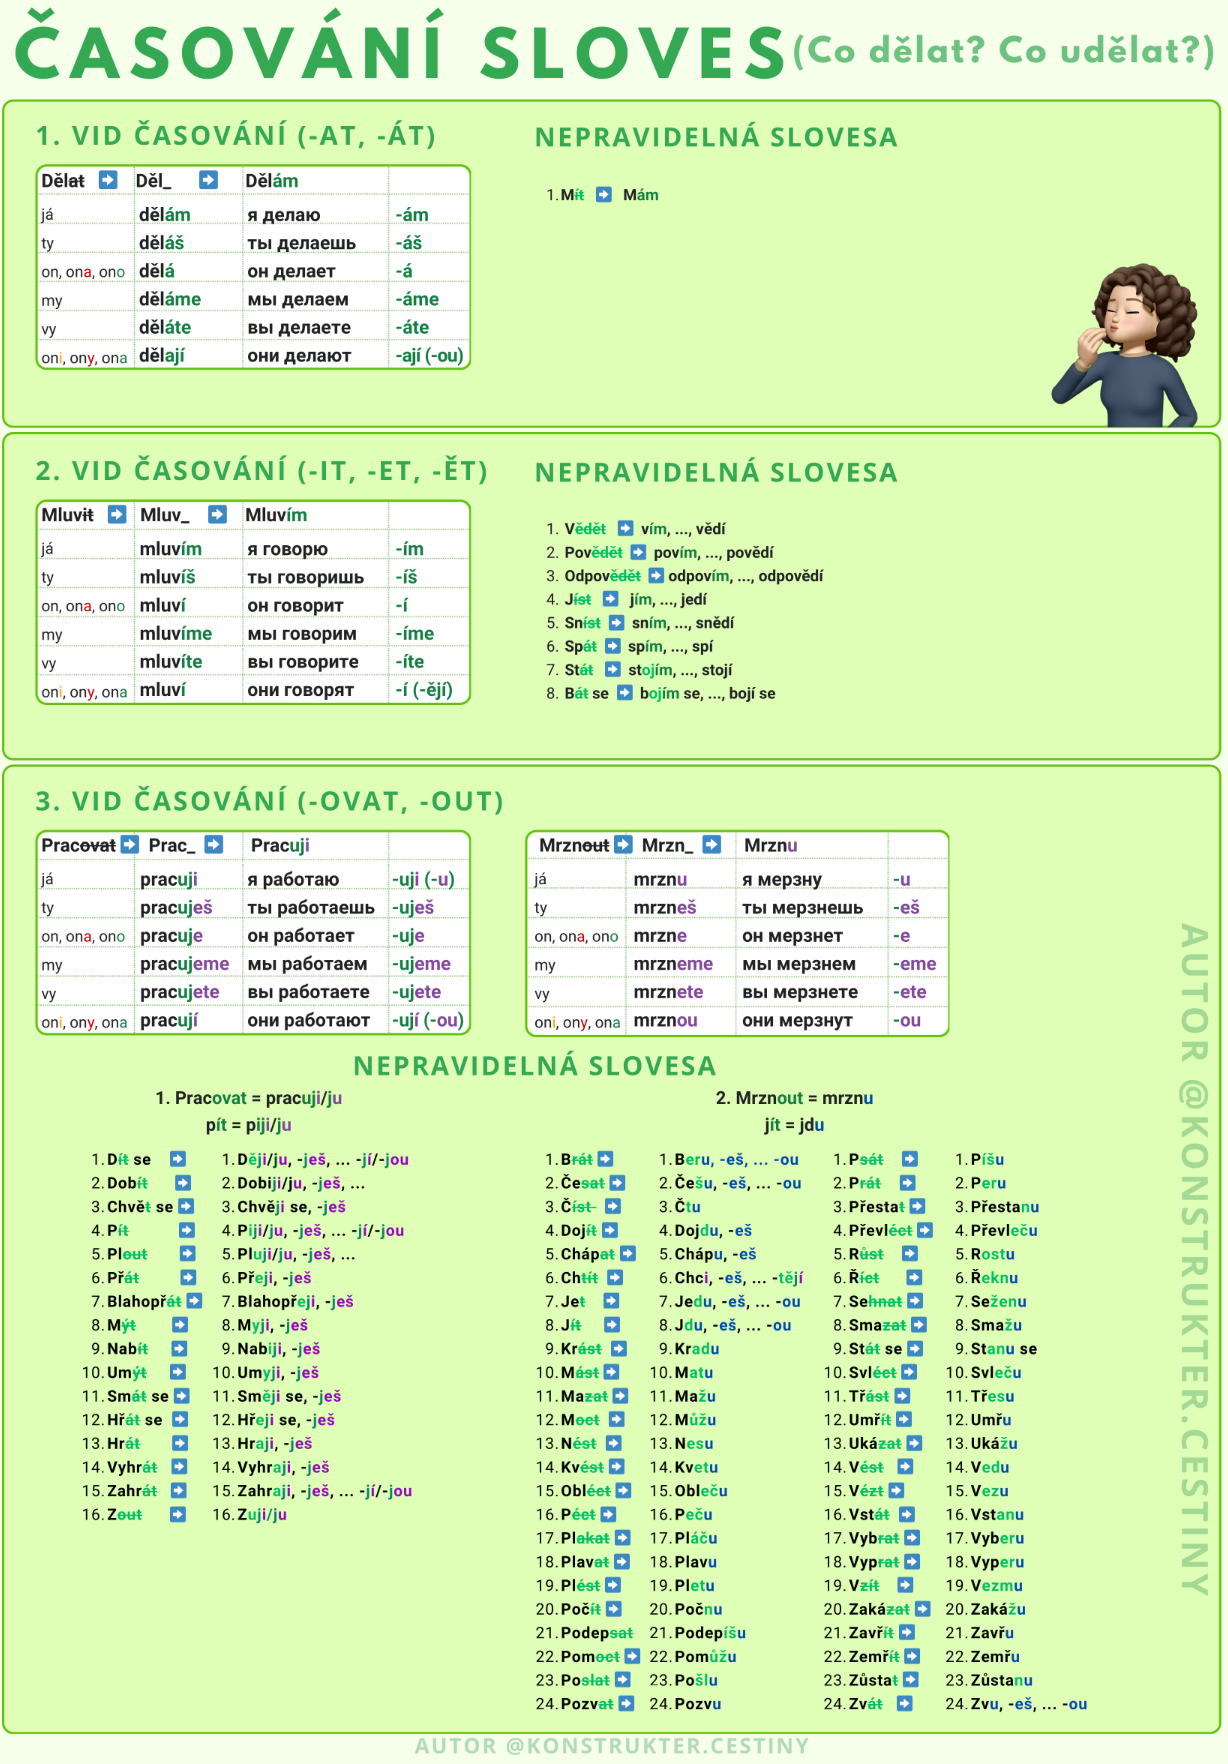
\includegraphics[scale=0.35]{Resources/casovani_sloves.png}
\caption{Časování sloves (conjugation of verbs)}
\label{fig:casovani_sloves}
\end{figure}

\clearpage

\section{Personal notes}
\subsection{Verb \emph{být}}
Figure~\ref{fig:verb_byt} illustrates the cases of verb \emph{být}.

\begin{figure}[h]
\centering
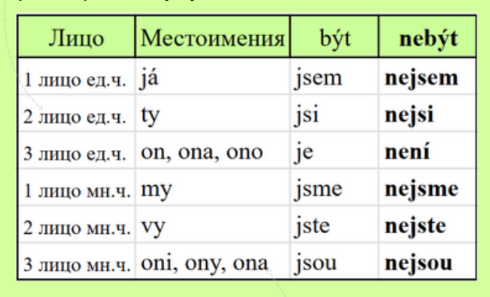
\includegraphics[scale=0.35]{Resources/verb_byt.png}
\caption{Verb být}
\label{fig:verb_byt}
\end{figure}

Important thing to notice are the verbs in the 3 case plural tense, where \textbf{oni} stands for \textbf{plural masculine} 
nouns, \textbf{ony} stands for \textbf{plural feminine} nouns, and \textbf{ona} stands for \textbf{plural neutral} nouns.

In the present tense, the verb \emph{byt} in the present tense is only present, when there are no other
verbs in the sentence, as it is illustrated on figure below.

\begin{figure}[h]
\centering
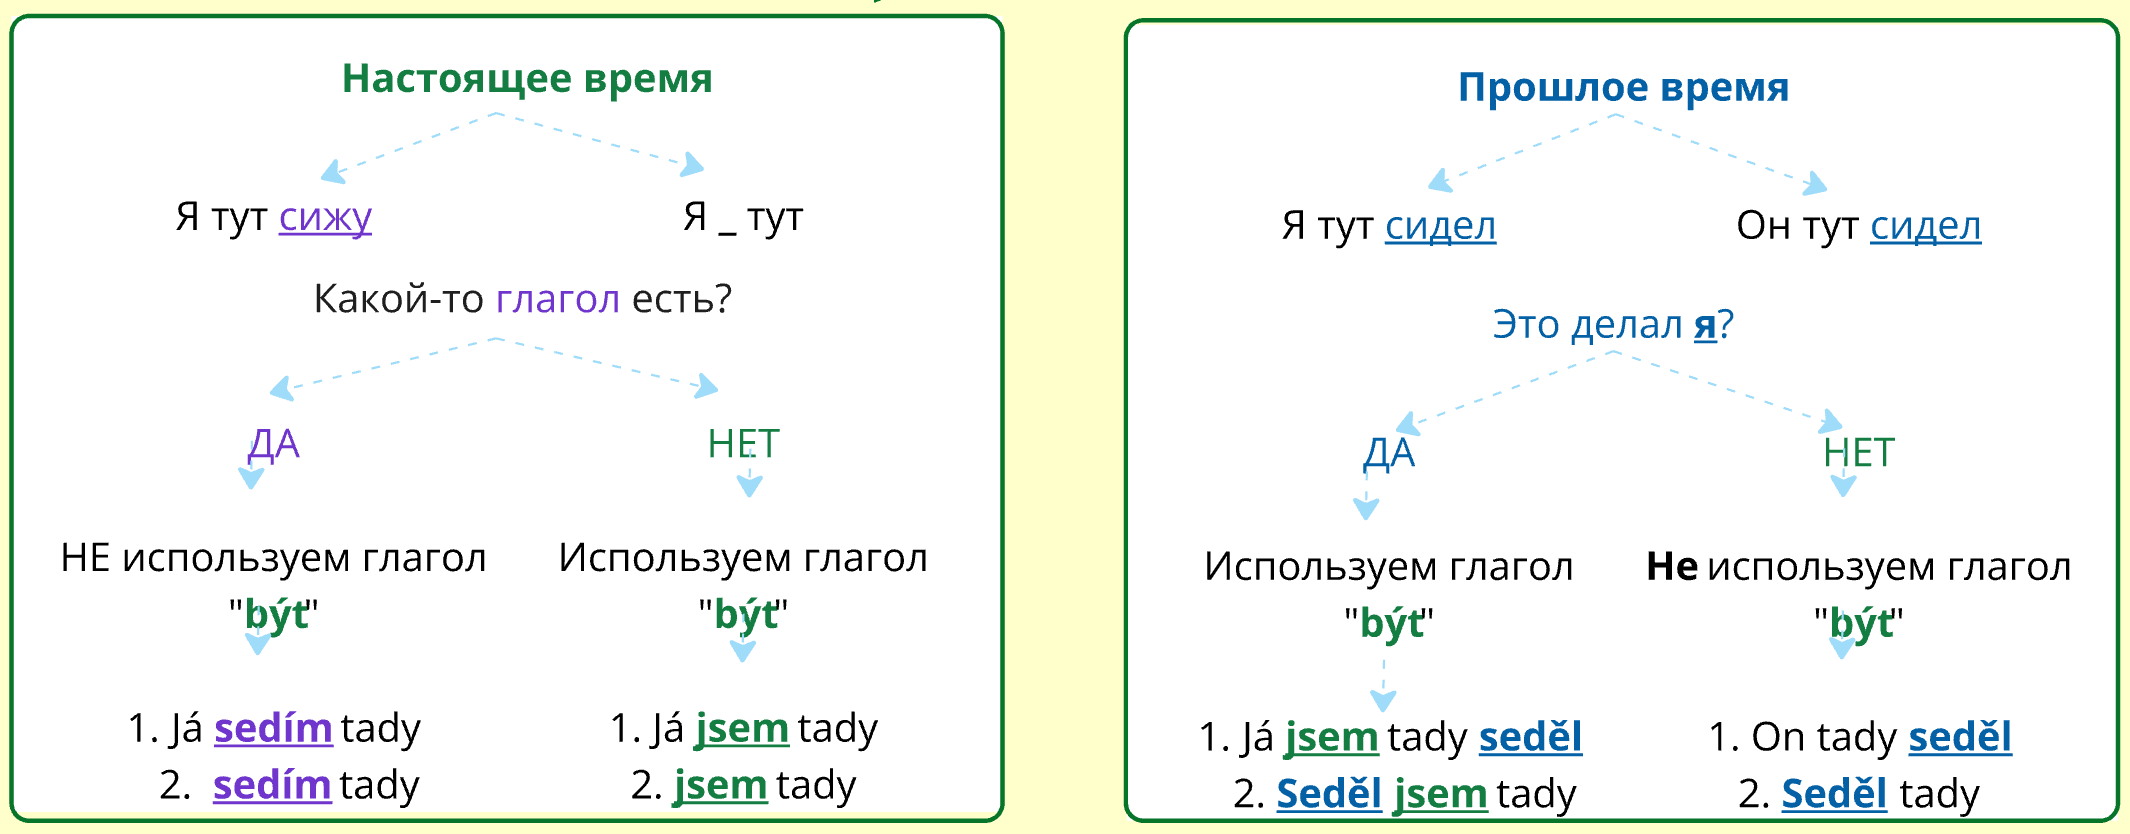
\includegraphics[scale=0.2]{Resources/verb_byt_in_present_past_tenses.png}
\caption{Verb byt in present and past tenses}
\label{fig:verb_byt_in_present_past_tenses}
\end{figure}

\subsection{Pronoun \emph{to}}
For saying that something is there, like \emph{it, the, that}, we use \textbf{ten} (masculine), \textbf{ta} (feminine), 
\textbf{to} (neutral).

For saying that something is close, like \emph{this}, we use \textbf{tento} (masculine), \textbf{tato} (feminine), 
\textbf{toto} (neutral).


\lecture{2}
If I like doing something or if it is healthy to do, then I use \emph{si} instead of \emph{se}.

Irregular verbs are the ones, which also change their root and not only the suffix, e.g. \emph{vědět} -- \emph{vím}.

Something large that ends in \emph{-ište}, e.g. \emph{parkovište}, then it is neutral or something natural \emph{odpoledne}.

Something smaller created by humans and nothing too large, e.g. \emph{televize}, \emph{lednice}, \emph{nemocnice}, is feminine.

Something like \emph{srdce} is also neutral, as it is not created by human.

Every noun that ends on \emph{-í} is neutral, e.g. \emph{nádobí}.

If the word has \emph{-tel} at the end, as \emph{přítel}, then is behaves as \emph{muž}.

\subsection{How to case nouns (\textrussian{спряжение по падежам})}
For correct casing of the noun (\textrussian(склонение по падежам)) we have to :
\begin{enumerate}
    \item Take the verb before that noun and find the correct case for the feminine singular and plural \textbf{žena}. 
        As the most important thing is to be able to know which case comes after the given verb.

    \item Find the exact table, from the gender tables below, where this noun refers to and conjugate it according to 
        the case we found in the first step.
\end{enumerate}

\begin{figure}[h]
\centering
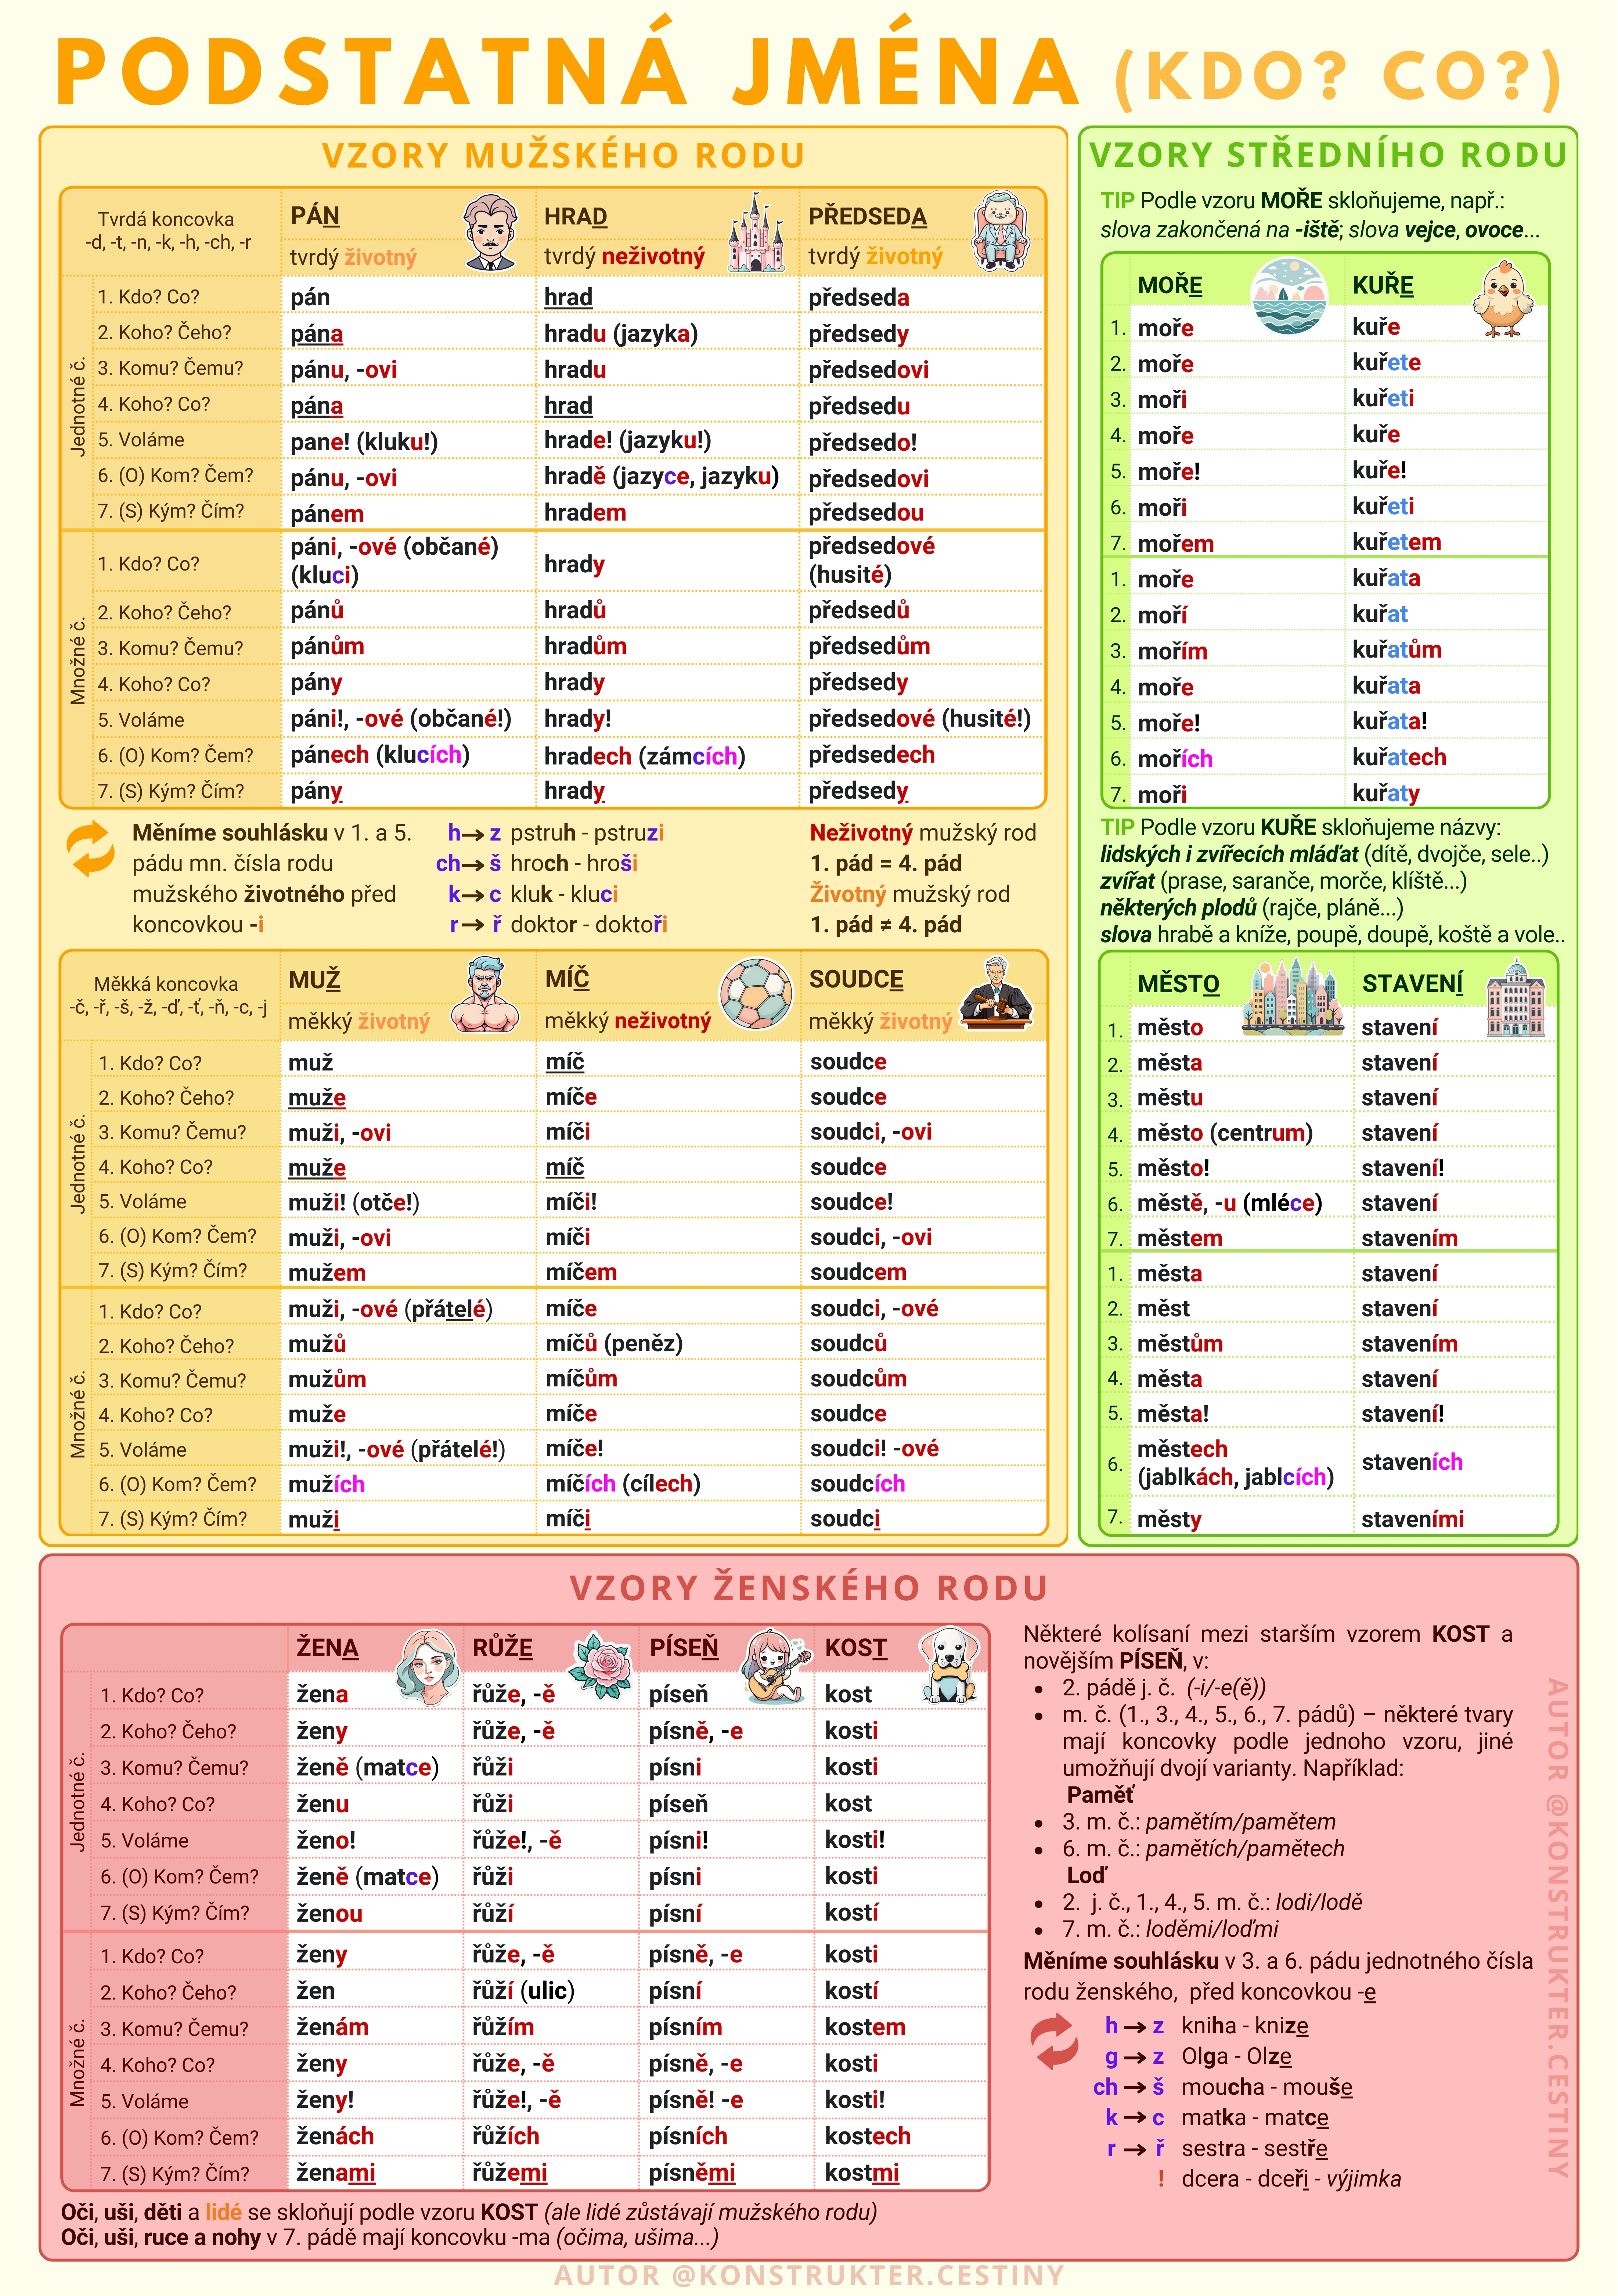
\includegraphics[scale=1]{Resources/nouns_conjugation.jpg}
\caption{Conjugation of nouns}
\label{fig:nouns_conjugation}
\end{figure}

\begin{figure}[h]
\centering
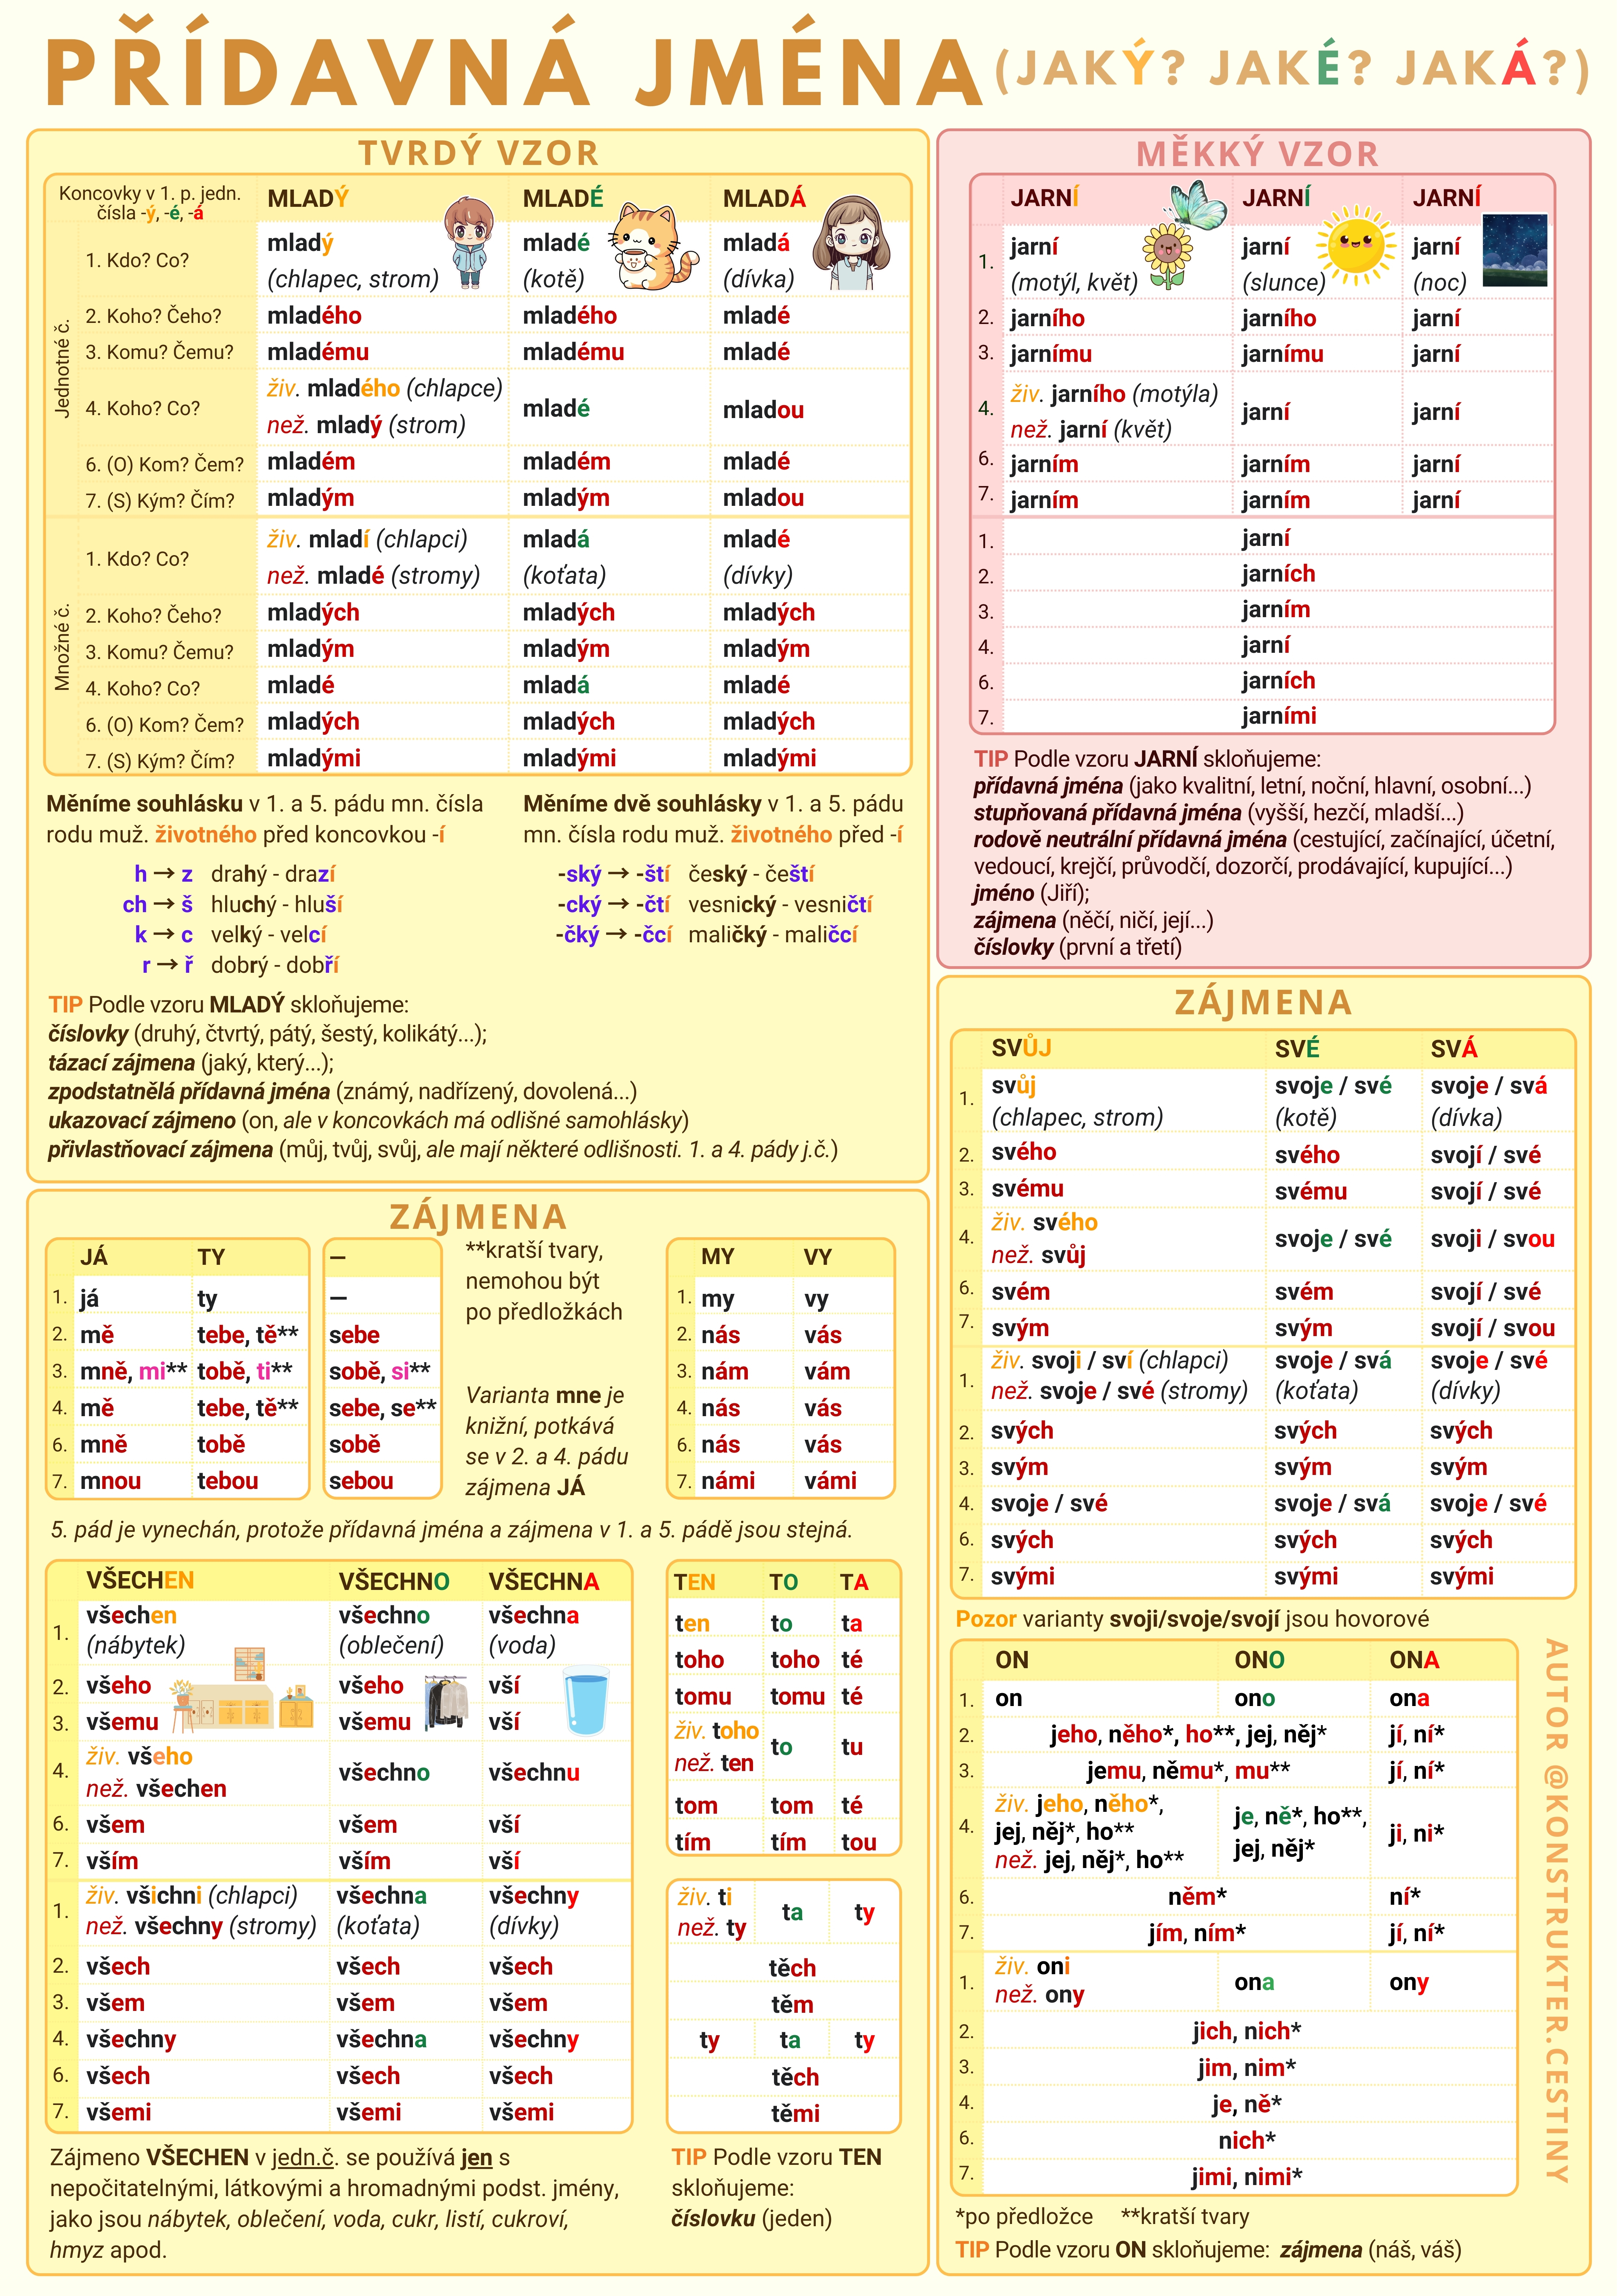
\includegraphics[scale=1]{Resources/adjectives_conjugation.jpg}
\caption{Conjugation of adjectives}
\label{fig:adjectives_conjugation}
\end{figure}



\lecture{3}
If we want to know if the noun is in the plural or not, we can look at the adjective before it also at its suffix 
to give us a hint of its case.

Adjectives like \emph{hodně}, \emph{malo}, \emph{vice}, \emph{mene}, \textrussian{то есть неисчислительные числительные}.

2 nouns together are usually in 2.nd case, e.g. \emph{uřad práce}.

Words coming from the latin language, e.g. \emph{muzeum}, are always in neutral gender.

After letter \emph{c}, there will never be \emph{a} or \emph{u}, but can be \emph{e} or \emph{i}.


\lecture{4}
In past tense, we don't add \emph{je} and \emph{jsou} for the 3rd person.

If the action comes back to me, then we use \emph{se}, e.g. \emph{učím se česky}.

Long \emph{ý} usually indicates an adjective, whereas short \emph{y} indicates on an adverb, e.g. \emph{český -- jaky? (jazyk)}, 
\emph{česky -- jak?}.

\begin{figure}[h]
\centering
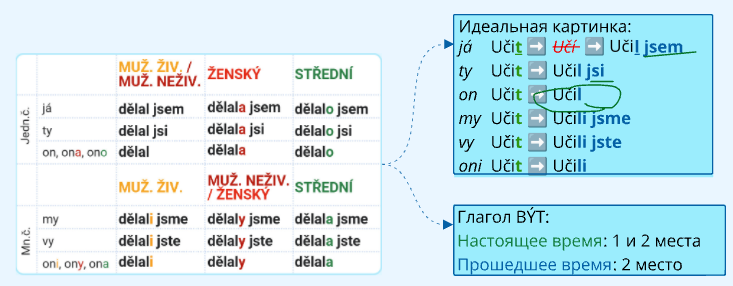
\includegraphics[scale=0.5]{Resources/past_tense.png}
\caption{Forming past tense}
\label{fig:past_tense}
\end{figure}

Below is illustrated how the verbs' suffixes change, when used in the past tense.

\begin{figure}[h]
\centering
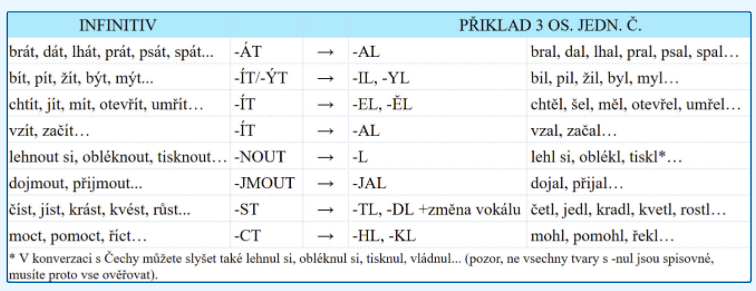
\includegraphics[scale=0.5]{Resources/past_tense_verbs.png}
\caption{Modification of verbs in the past tense}
\label{fig:past_tense_verbs}
\end{figure}

Below are the incorrect words that change the root in the past tense.

\begin{figure}[h]
\centering
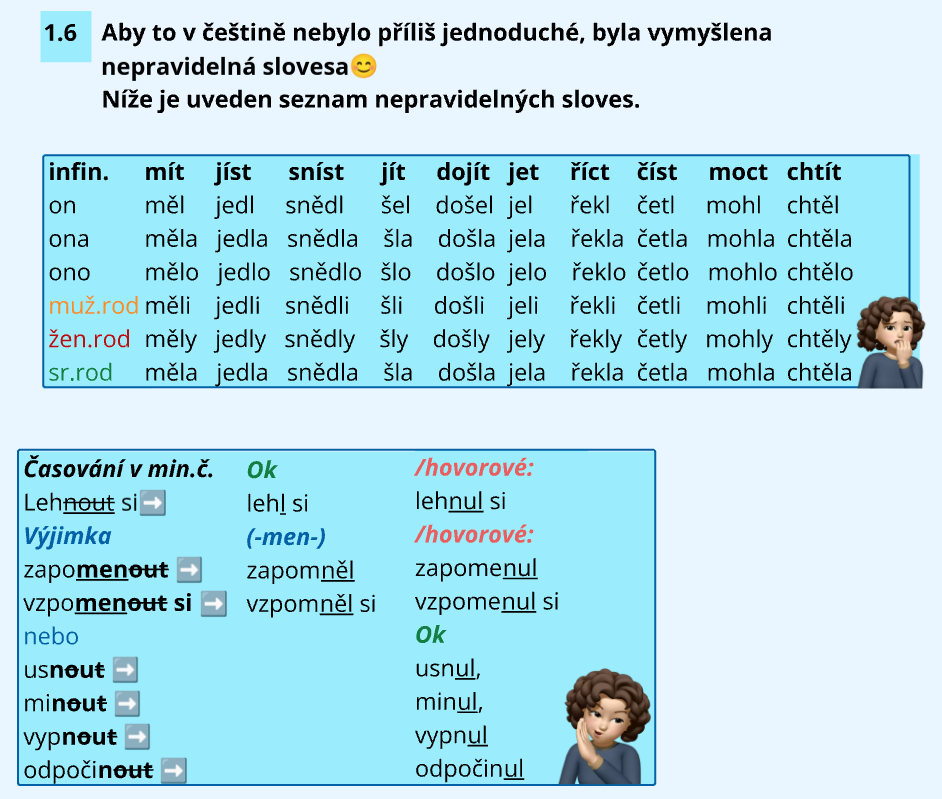
\includegraphics[scale=0.4]{Resources/incorrect_words_past_tense.png}
\caption{Incorrect words past tense}
\label{fig:incorrect_words_past_tense}
\end{figure}

Figure below illustrates how verbs change in past tense, including the usage of words 
\emph{bych}.

\begin{figure}[h]
\centering
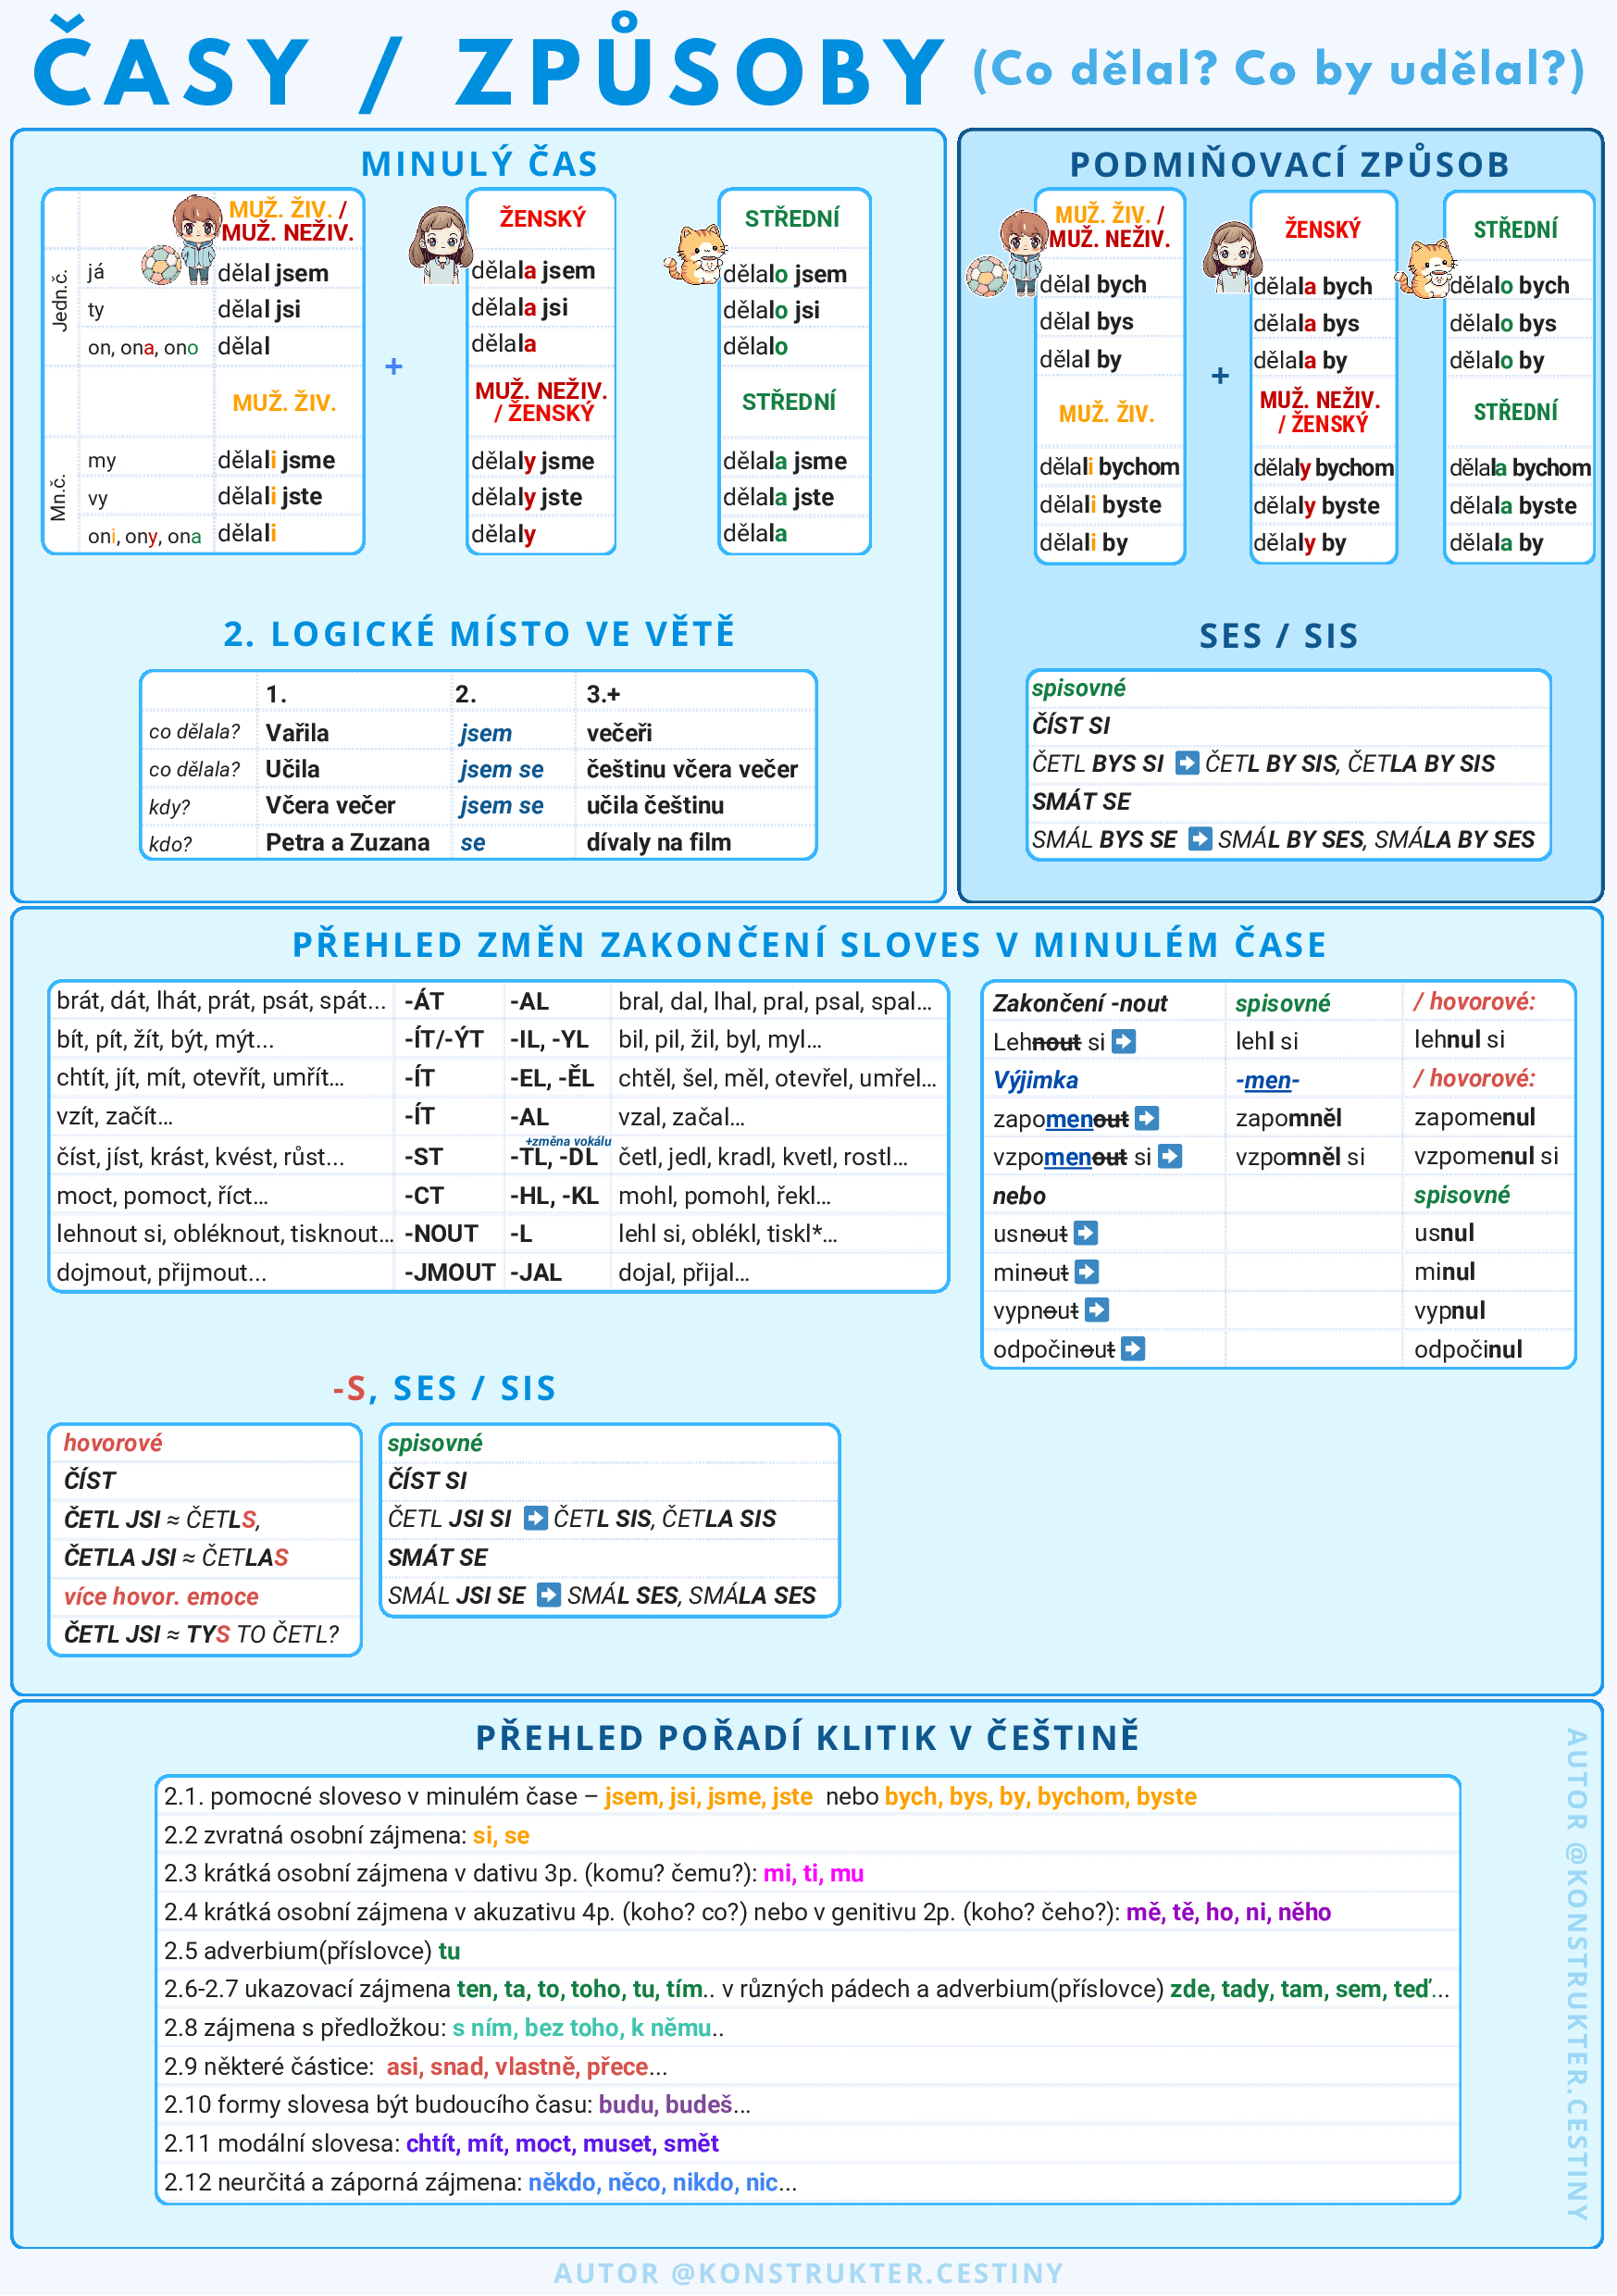
\includegraphics[scale=0.2]{Resources/casy_zpusoby.png}
\caption{Časy/způsoby}
\label{fig:casy_zpusoby}
\end{figure}


\lecture{5}
If we want to use \emph{mám rád} then there should come a noun, but if we want to use \emph{rád neco udelat}, i.e. with the verb,
then we don't use \emph{mám}.

From somewhere, then we use \emph{z}: \emph{jsem z Azerbajdžanu}, and if we are with someone, then we say \emph{s}: \emph{s kamarády}.

When we use \emph{by} in past tense, then we don't need \emph{jsem} or \emph{jste} anymore, e.g. \emph{jedl bych do kina}.


\lecture{6}
If we go inside some place, we say \emph{do}, e.g. \emph{do kavarny}. If we say that we go to some open place, 
e.g. square, we say \emph{na}, e.g. \emph{na náměstí}, or to some sightseeing or event, e.g. \emph{do diskotéki}. If we say that we 
are going inside some important established institution (official places), e.g. ministry, post-office, University, we also say 
\emph{na}, instead of \emph{do}, e.g. \emph{do ministerstva vnítra}.

For regions, we would use \emph{na}, e.g. \emph{na Moravě}, but for cities, we use \emph{v}, e.g. \emph{v Brne}.

If I am inside a place and get out from there, then I say \emph{z}, e.g. \emph{z metra}, but if I go from outside of some place,
then I say \emph{od}, e.g. \emph{od metra} (from outside the metro).

Preposition \emph{s} has to do with the 7-th case (\emph{kým? čím?}), whereas preposition \emph{z} has to do with the 2-nd case 
(\emph{kodo? čeho?}).

\begin{figure}[h]
\centering
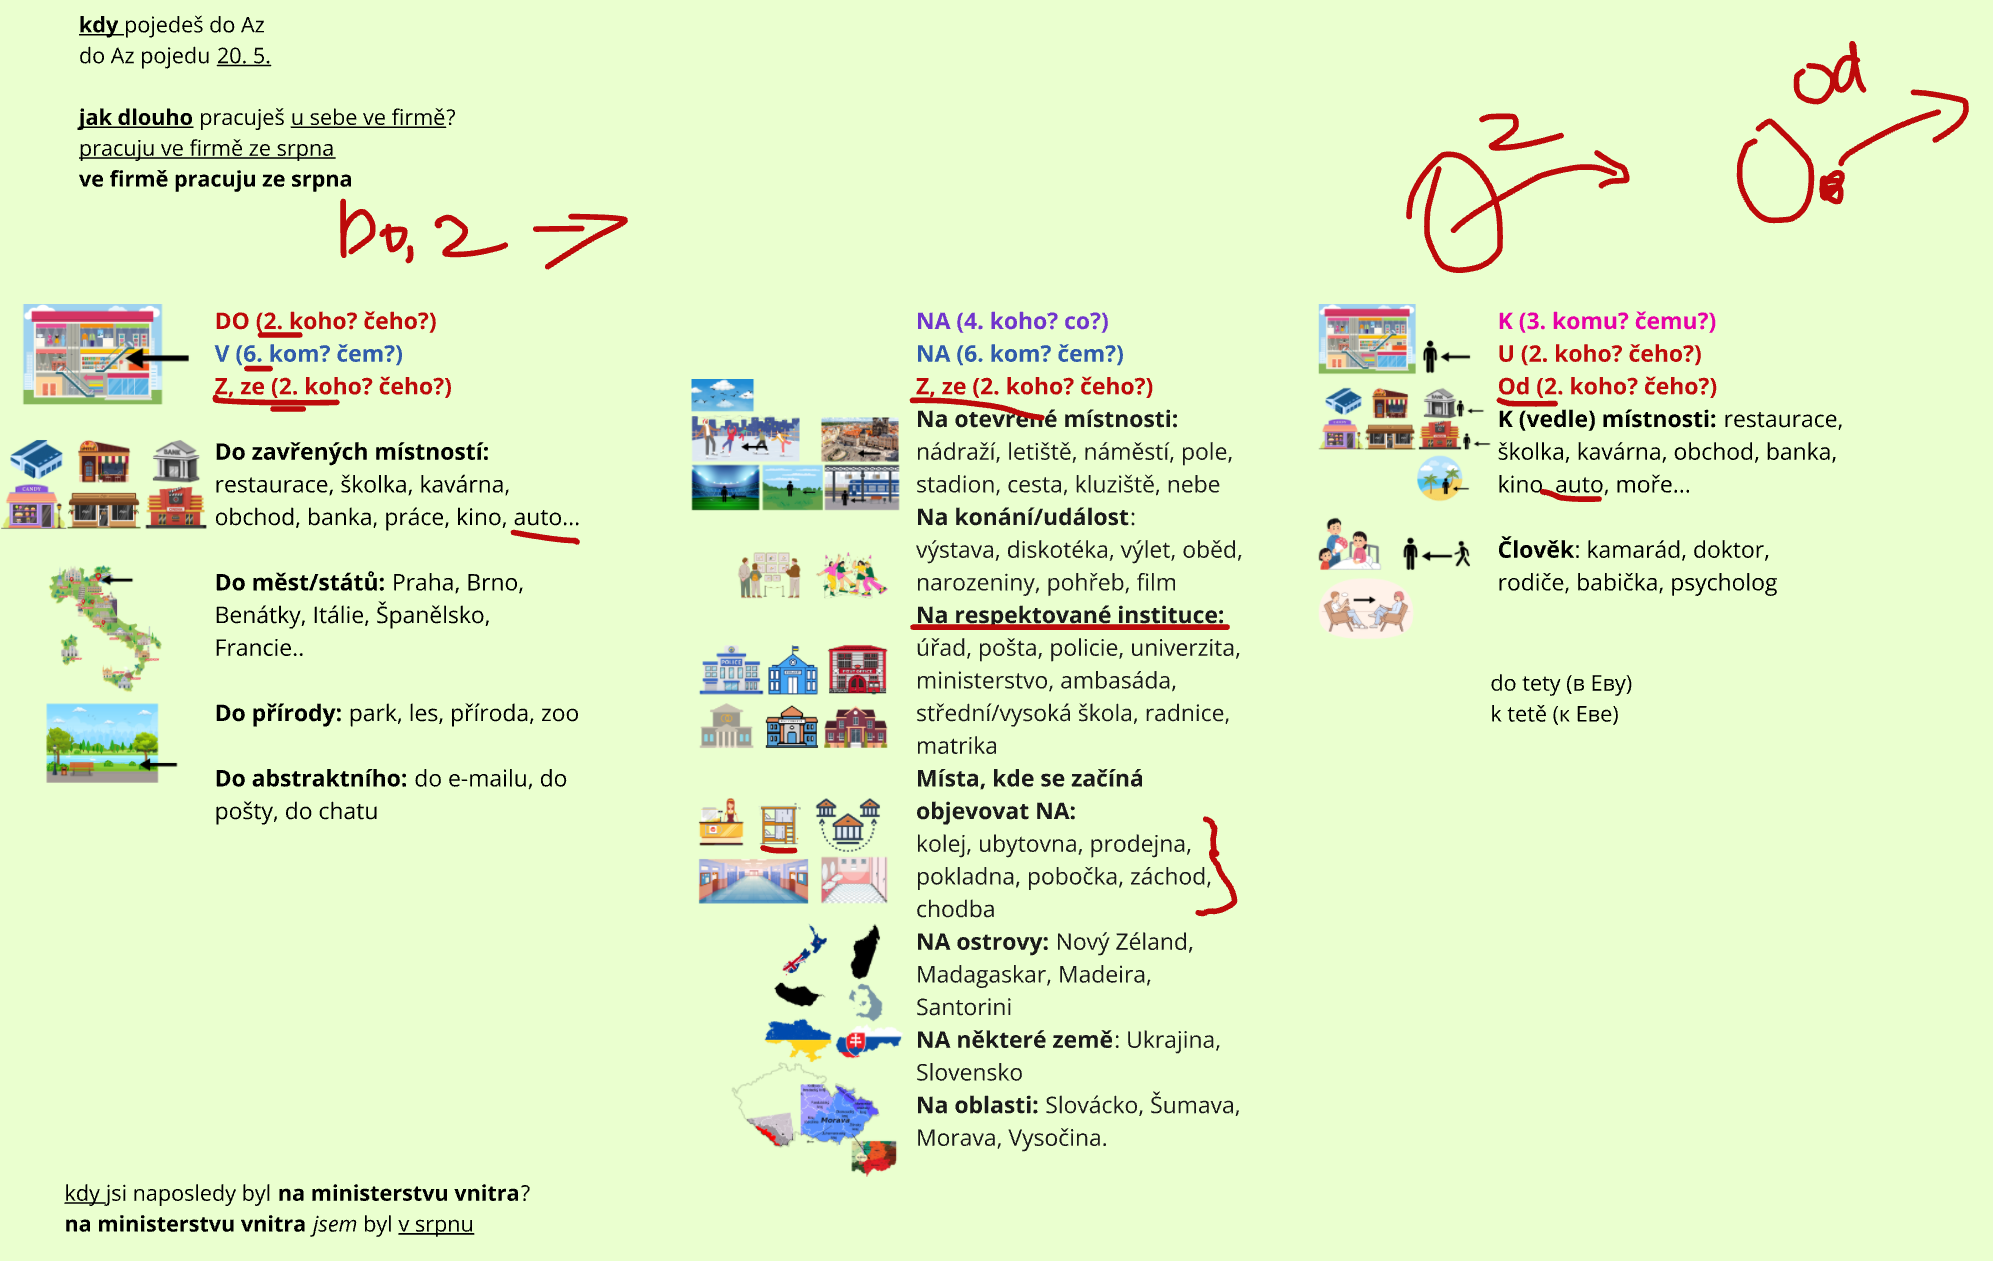
\includegraphics[scale=0.25]{Resources/place_prepositions.png}
\caption{Place prepositions}
\label{fig:place_prepositions}
\end{figure}


\lecture{7}
With masculine and animate we say \emph{všichni}, but with feminine, neutrum, and inanimate, we use \emph{všechny}.

In future tense, we can either:
\begin{itemize}
    \item With \emph{budu} + infinitive, e.g. \emph{budu dělat}. This means that I will do it in the future without 
        guarantee of finishing it.
    
    \item With adding prefices \emph{do, po, u}, e.g. \emph{udělat}. This means that I will do it once in the future and will 
        finish it.
\end{itemize}

\begin{figure}[h]
\centering
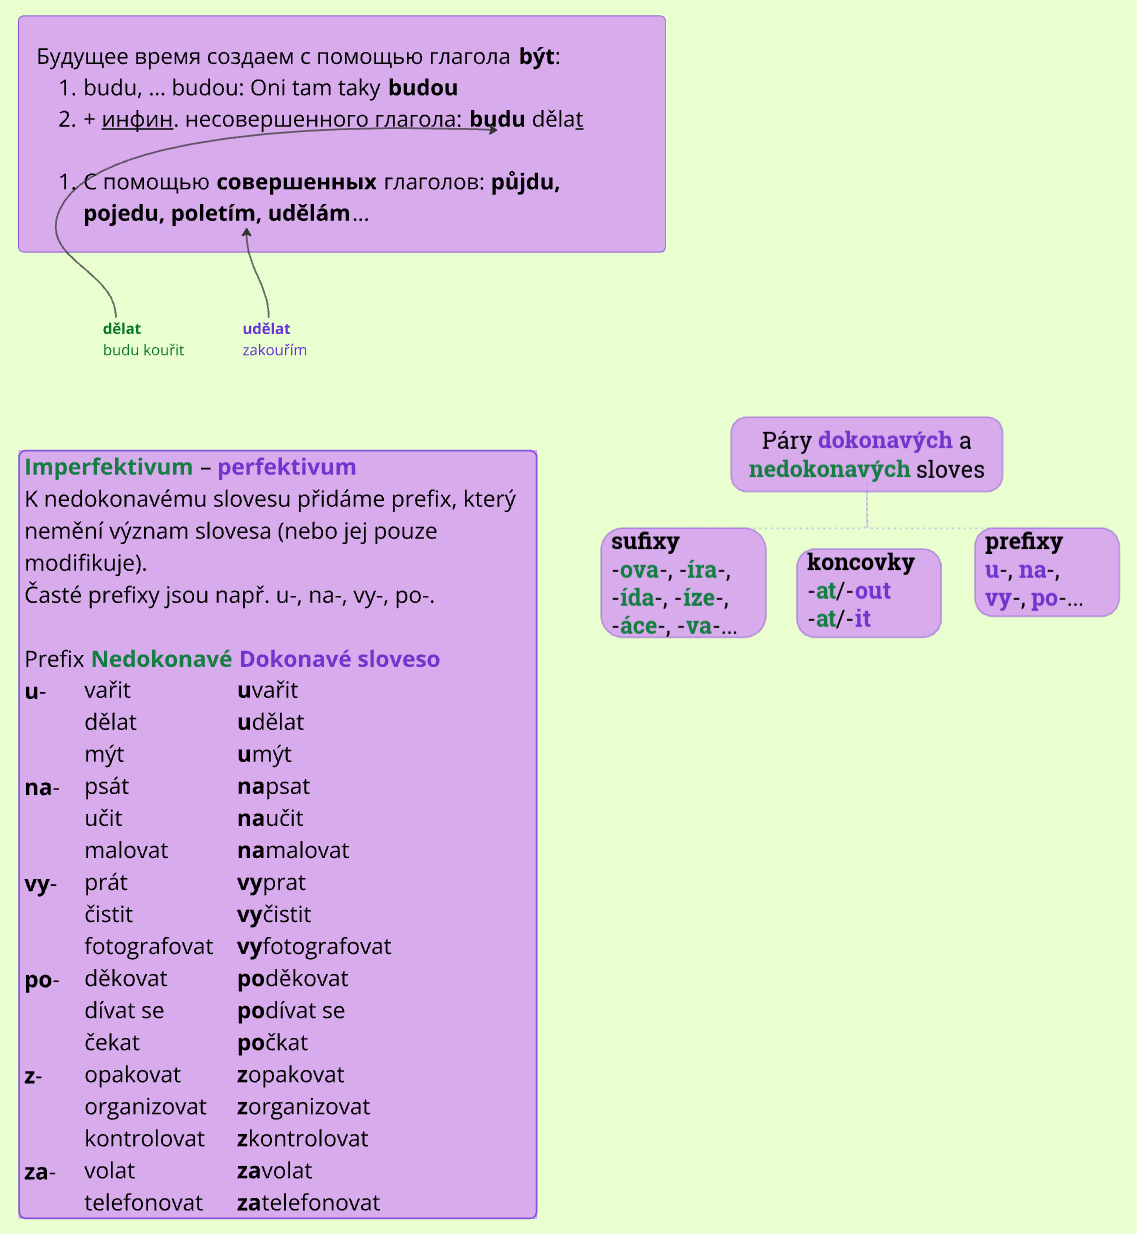
\includegraphics[scale=0.3]{Resources/future_tense.png}
\caption{Future tense}
\label{fig:future_tense}
\end{figure}

\begin{figure}[h]
\centering
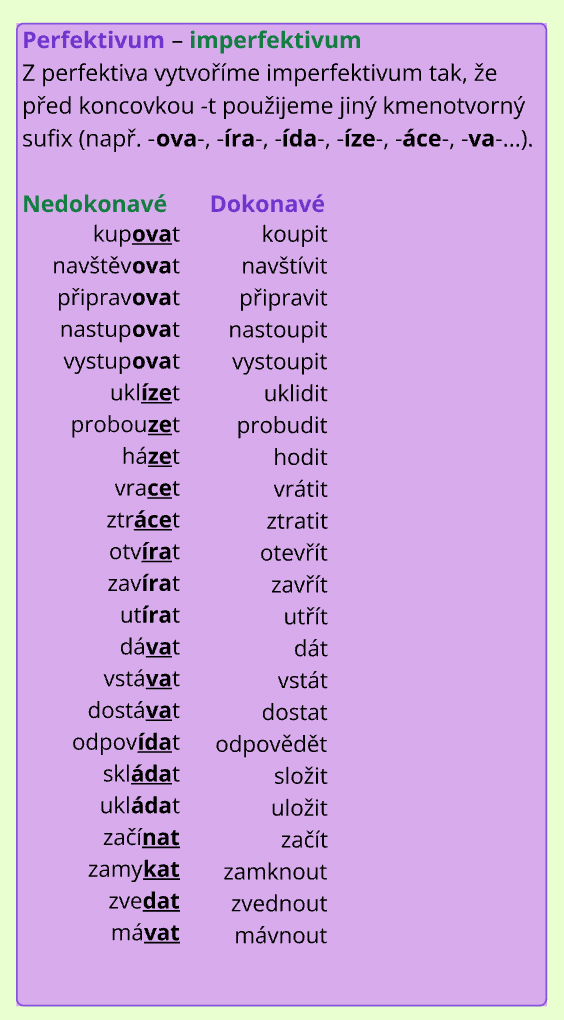
\includegraphics[scale=0.4]{Resources/perfect_to_imperfect_verbs.png}
\caption{Perfect to imperfect verbs}
\label{fig:perfect_to_imperfect_verbs}
\end{figure}


\lecture{8}
With irregular verbs, all the consonants are shortened, i.e. not long ones, e.g. \emph{pít -- pije}.

To find out the gender, we have to do these steps:
\begin{enumerate}
    \item Ask the question \emph{ten? ta? to?}.
    \item If it is masculine, then find out if it is animate or inanimate.
    \item Check the suffix, i.e. ending, to find out which example it relates to.
    \item Ask the question \emph{bez koho? čeho?}.
\end{enumerate}

Difference between the feminine words ending with \emph{e} and neutral ones ending with \emph{e}, is that the neutral one
is something very large and natural, e.g. \emph{moře}, whereas feminine is something smaller, e.g. \emph{růže} or \emph{sklenice}.

When words end with \emph{um}, e.g. \emph{centrum, vízum}, or with \emph{ma}, e.g. \emph{téma, aroma, karizma, panorama}, 
these are foreign words and they are in neutral gender. Figure below illustrates the conjugation of such words.

For \emph{muzeum} in the 6th pad we will have \emph{muzeích} and not \emph{muzeech}, as there is already a consonant \emph{e}.

All wrong neutral gender words, e.g. koma, téma, get \emph{at} as a suffix, e.g. \emph{tématu}, \emph{komatu}, \emph{panorámatu}.

\begin{figure}[h]
\centering
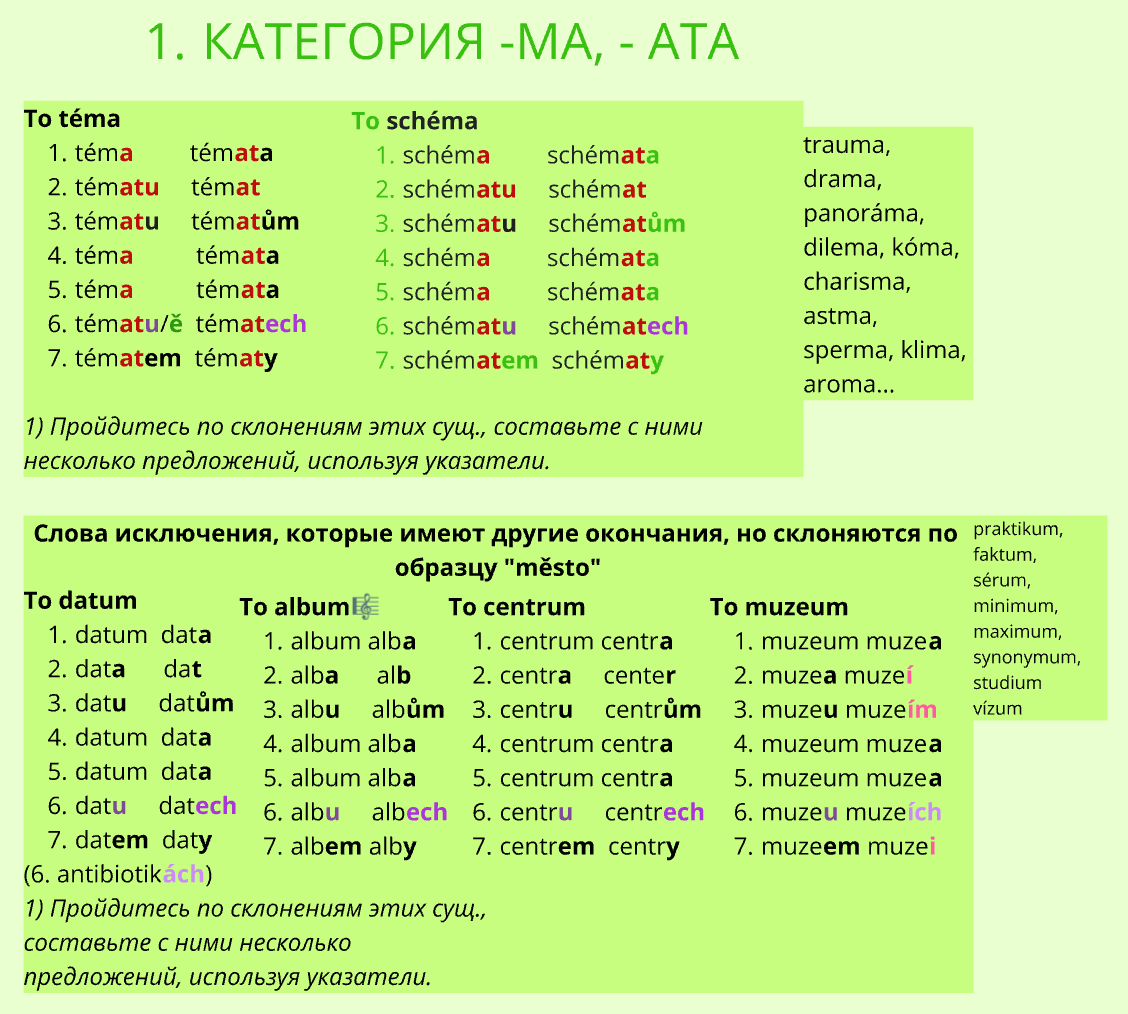
\includegraphics[scale=0.35]{Resources/special_neutral_gender_words.png}
\caption{Special neutral gender words}
\label{fig:special_neutral_gender_words}
\end{figure}


\lecture{9}
When we want to conjugate the date, e.g. 31st of May, we say \emph{třicatého prvního páty}, so numbers 1 and 3 conjugate as 
\emph{jarní}, but the rest conjugate as \emph{mladý}. But we don't conjugate the month, e.g. \emph{páty} stays the same.


\lecture{10}
\emph{Se} and \emph{si} are actually pronouns, they are substitutes for \emph{sobě} and \emph{sebe}.

\begin{figure}[h]
\centering
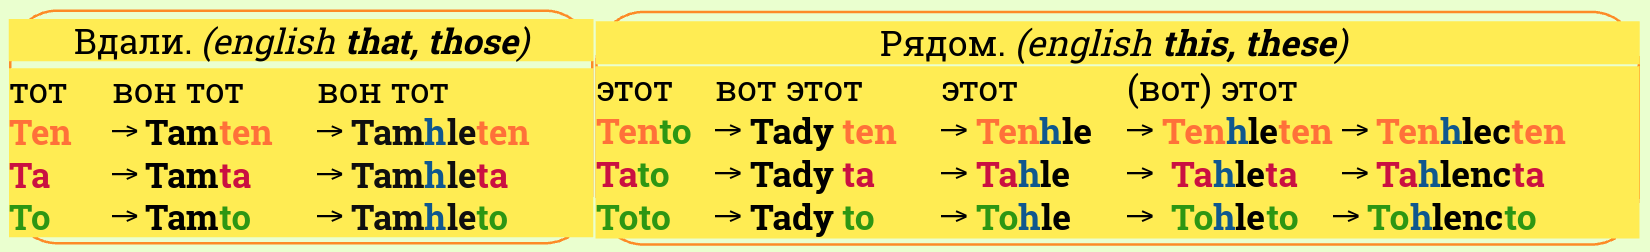
\includegraphics[scale=0.25]{Resources/ten_ta_to.png}
\caption{Ten, ta, to}
\label{fig:ten_ta_to}
\end{figure}


\lecture{11}

\begin{figure}[h]
\centering
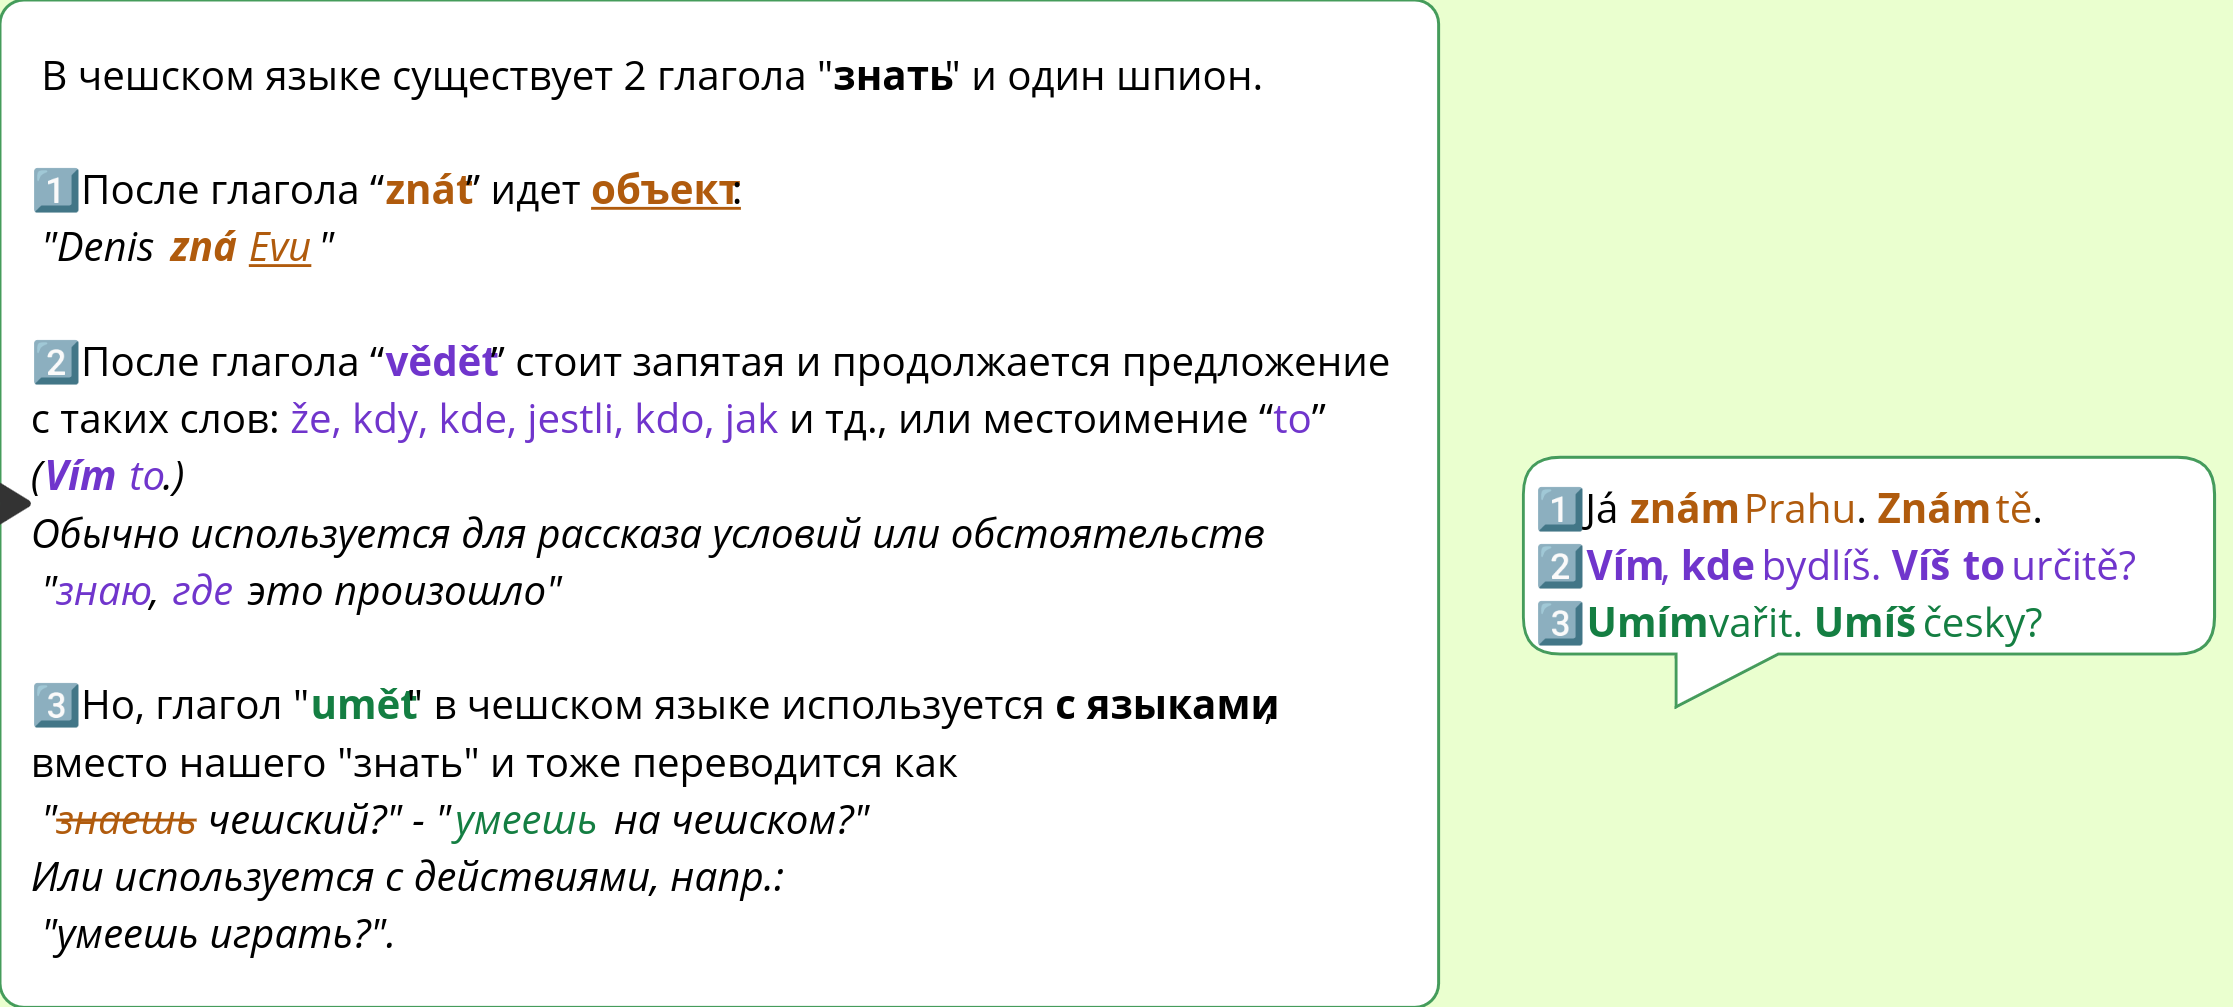
\includegraphics[scale=0.175]{Resources/znat_umet_vedet.png}
\caption{Difference between znát, vědět, umět}
\label{fig:znat_umet_vedet}
\end{figure}


\lecture{14}
If I say \emph{Jeho boli hlava}, because of that \emph{jeho}, I can put it to the beginning of the sentence.
But if I said \emph{boli ho hlava}, because of that \emph{ho}, we have to put it to the second logical place in the sentence.

\begin{figure}[h]
\centering
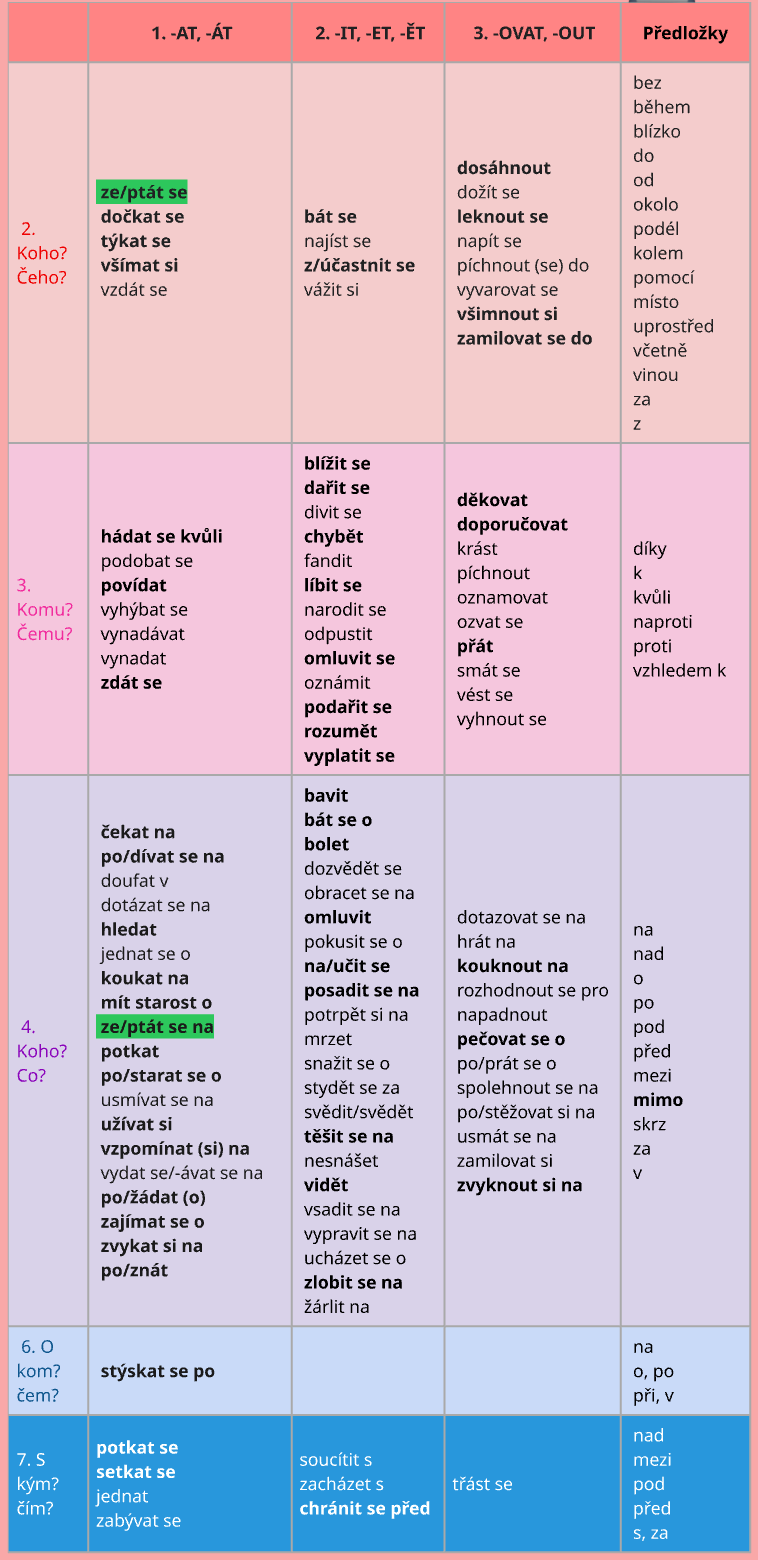
\includegraphics[scale=0.4]{Resources/predlozky_a_pady.png}
\caption{Předložky a pady}
\label{fig:predlozky_a_pady}
\end{figure}


\lecture{15}
If we want to say older by 2 years, we would say \emph{starši o dva roky}.

Usually after prepositions \emph{v, ve}, we use nouns in locative case, but with handful of exceptions,
e.g. days of the week (\emph{v neděle}) or believing into something hoping for something (\emph{veřim v Boha}),
the noun that comes after prepositions \emph{v, ve} is in accusative case.

When we are talking about hours or minutes, i.e. \emph{v 9 hodin} or \emph{trvají 80 minut}, 
if time is less than 5, i.e. 2, 3, 4 (except for 1, as after 1 we use noun in nominative case (kdo? co?)),
we use accusative plural case (\emph{koho? čeho?} in plural), e.g. \emph{v 12, 13, a 14 hodin}, 
but with numbers 5+ we use noun in genitive case plural form, e.g. \emph{v 2 hodiny}.

\lecture{16}
Word 1 \emph{jeden}, conjugates as word \emph{ten}.

Word 2 \emph{dva, oba}, conjugates like word \emph{koleno}.

Word 3 and 4 \emph{tři, čtyři}, conjugate a lot like word \emph{kost}.

With words 5 and 10 \emph{pět, deset}, simply add \emph{i} at the end.

\begin{figure}[h]
\centering
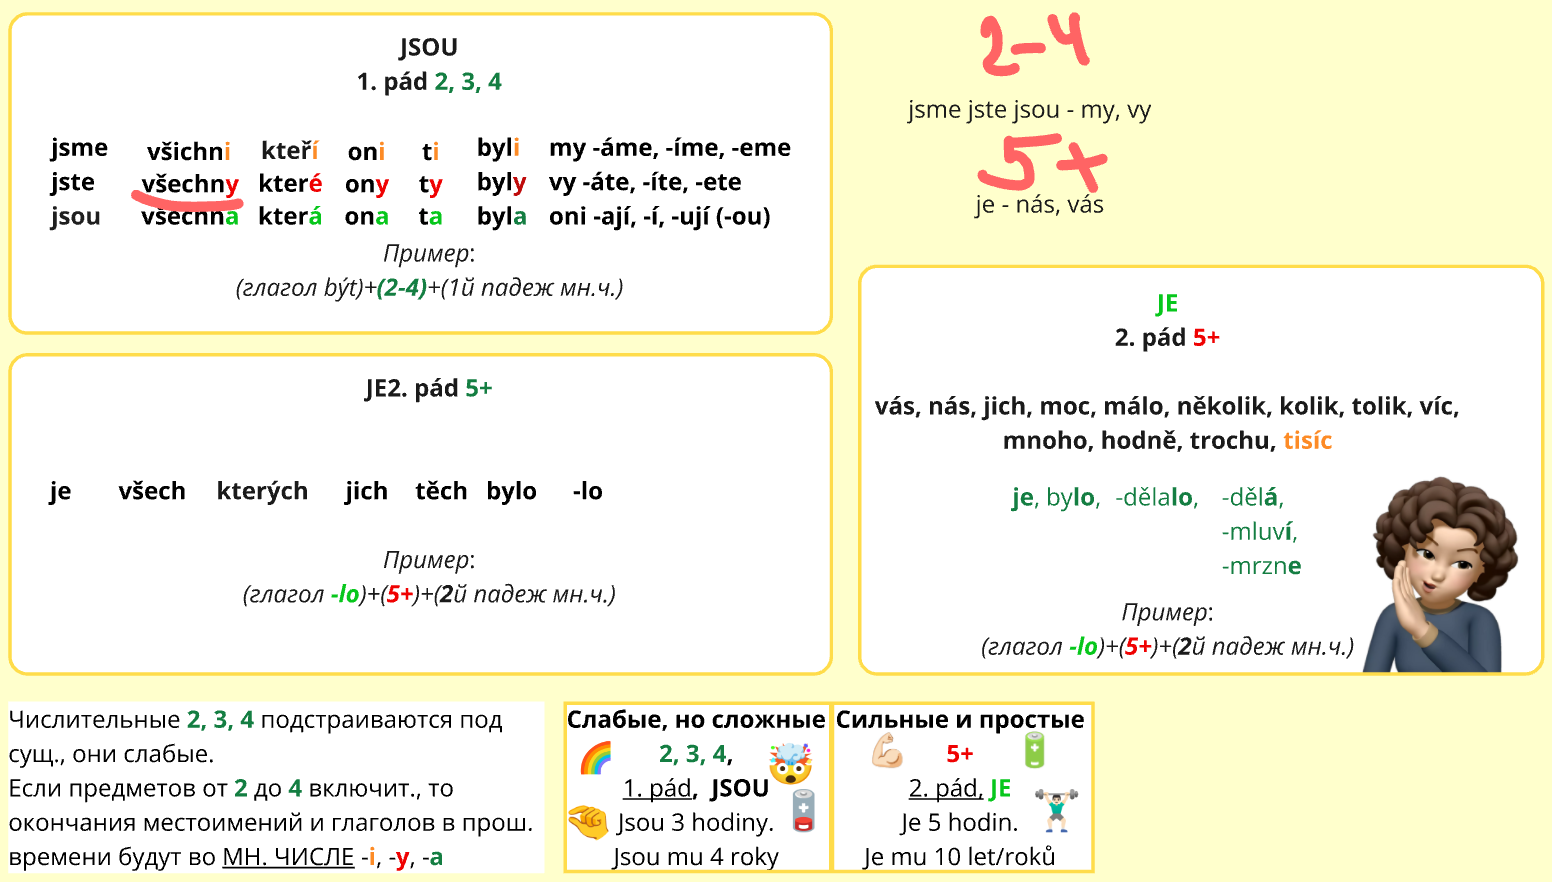
\includegraphics[scale=0.275]{Resources/cislovky_1.png}
\caption{Čislovky}
\label{fig:cislovky_1}
\end{figure}

\begin{figure}[h]
\centering
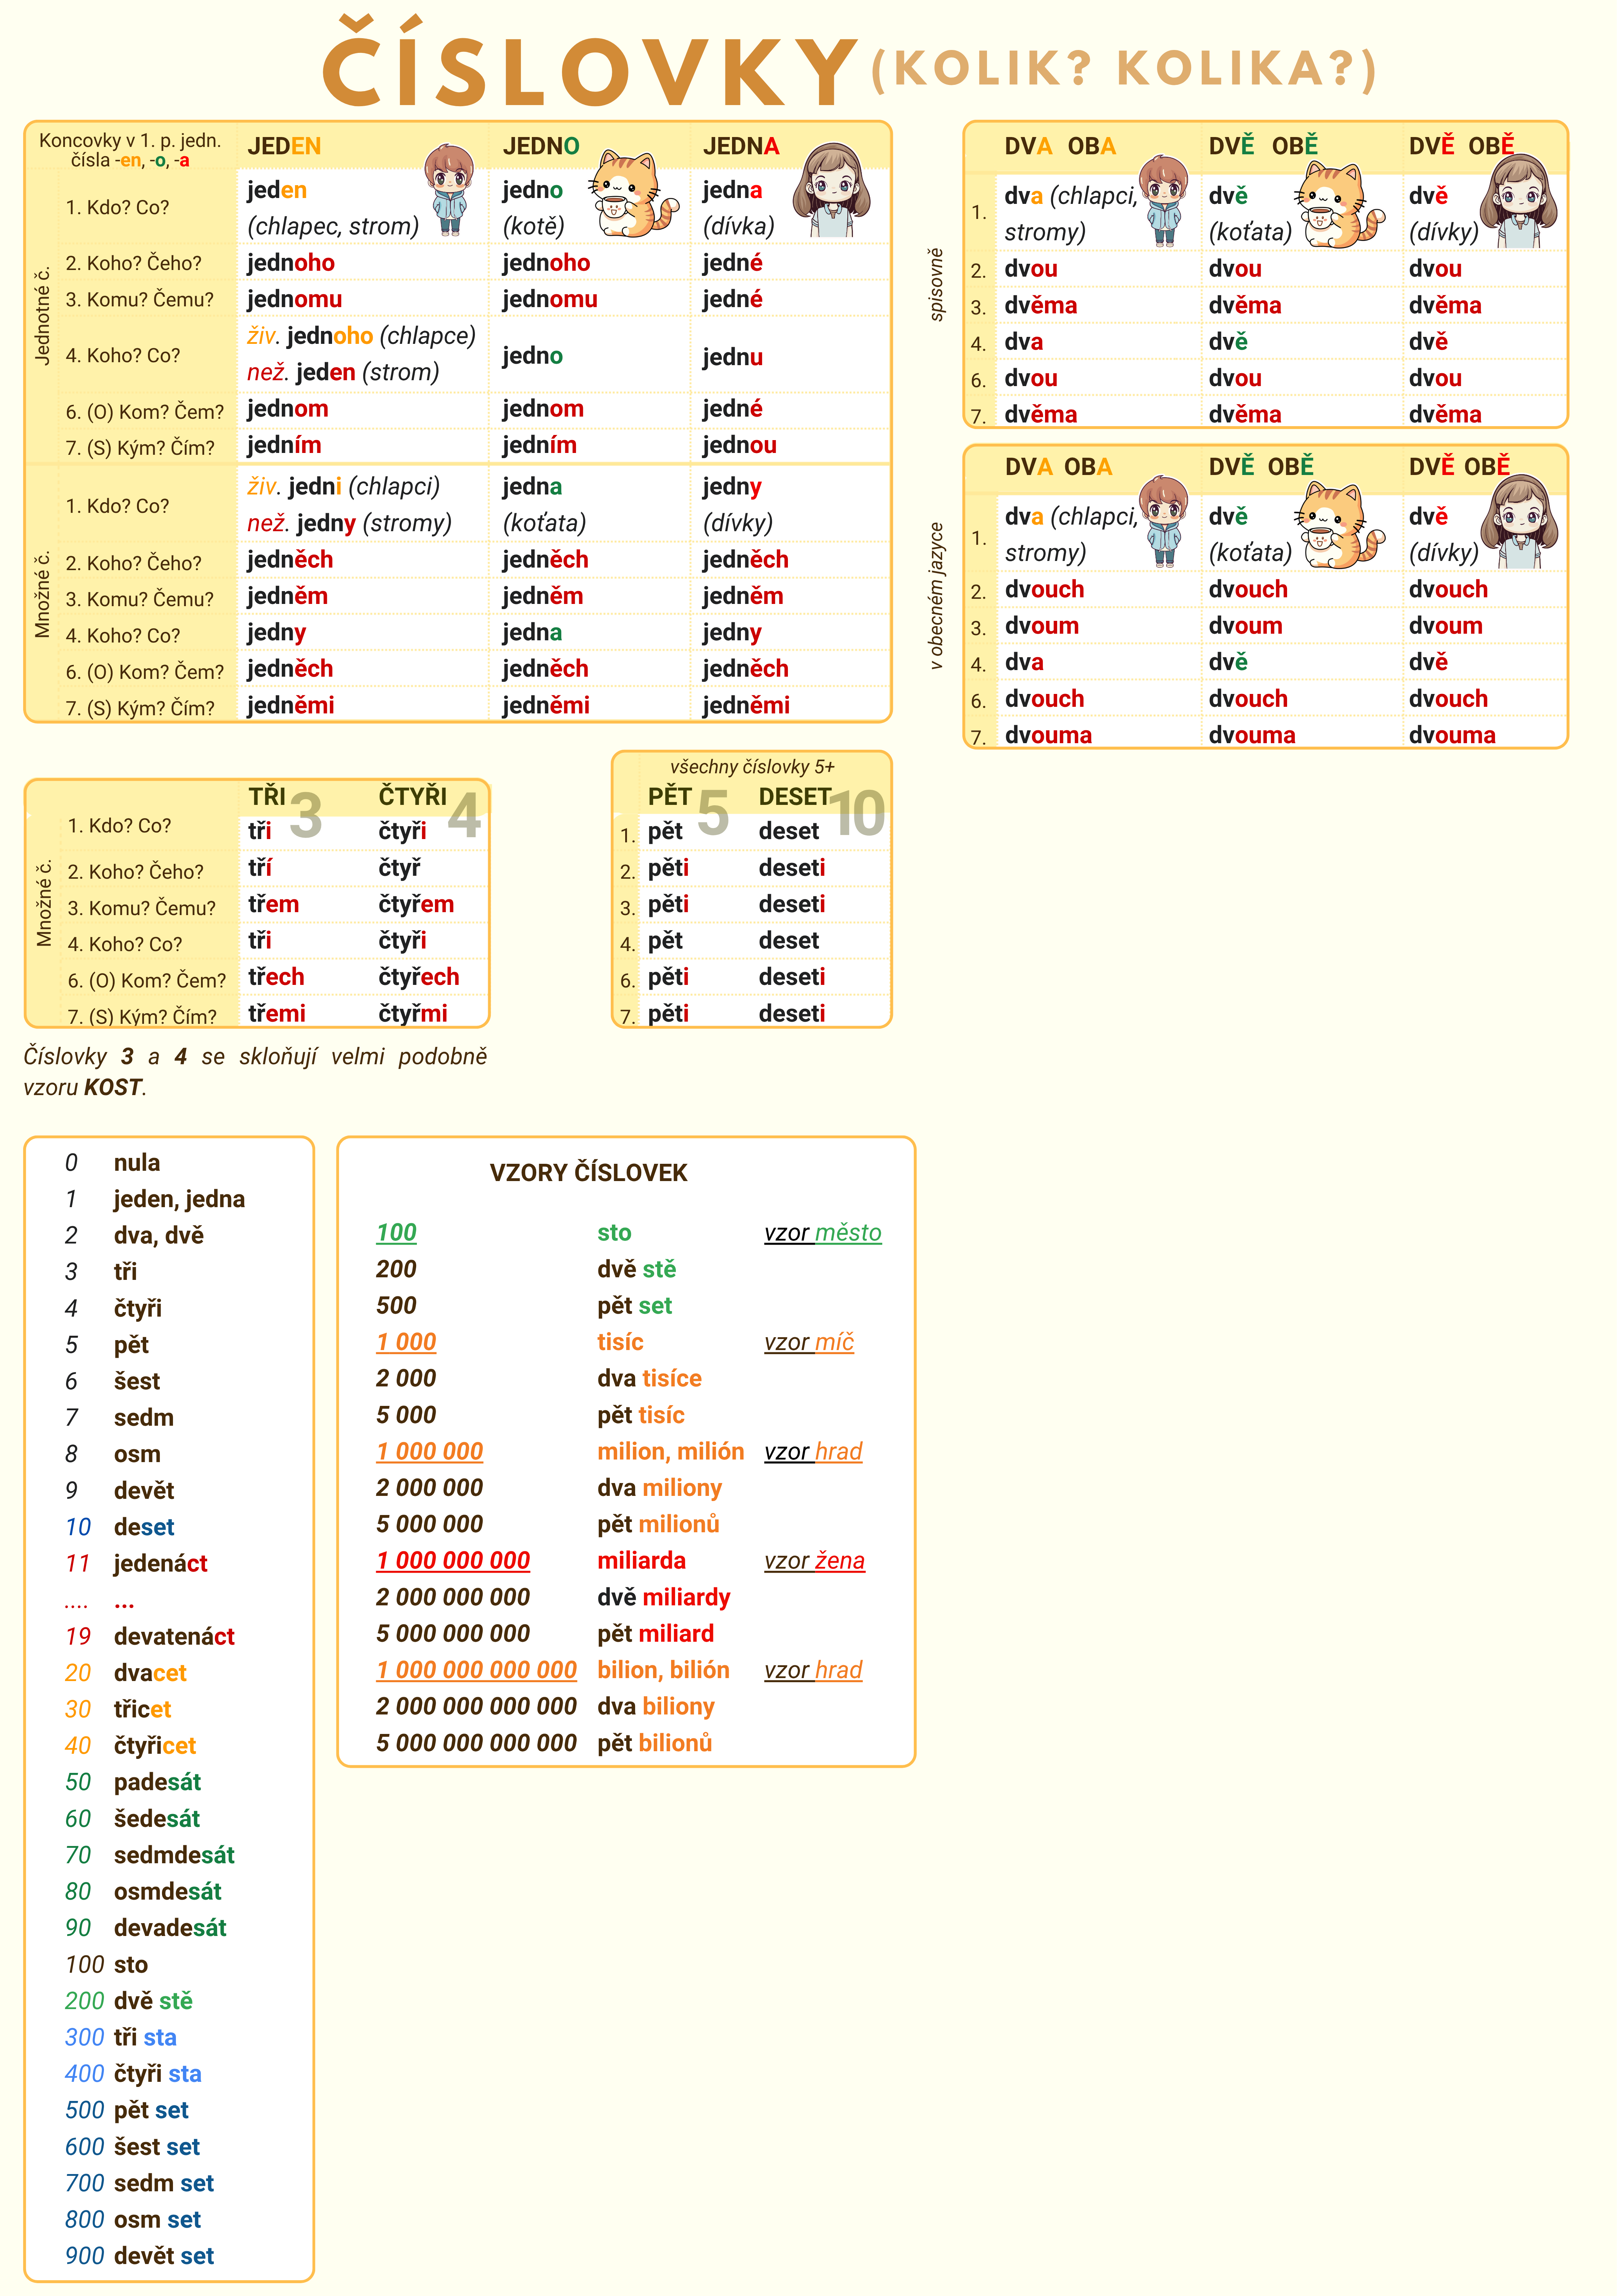
\includegraphics[scale=1]{Resources/cislovky_2.png}
\caption{Čislovky}
\label{fig:cislovky_2}
\end{figure}

Ordered numbers \emph{řadove čislovky} like \emph{druhý, čtvrtý, pátý, šestý, kolikátý} decline like \emph{mladý},
whereas \emph{první, třetí} decline like \emph{jarní}.

Dates are ordered numerals in genitive case, e.g. \emph{dvacatého třetí srpna} (23rd of August).


\lecture{17}
When we are talking about the future tense, \emph{když} means $50\%$ (it is like \emph{jestli} 
in future tense), but \emph{až} means that an action will happen with $90\%$ probability.

In 3rd case (dative), we could use either \emph{mně} or \emph{mi}, based on the rules illustrated on the 
figure below. The rules apply between \emph{tobě} and \emph{ti} and between \emph{sobě} and \emph{si}.

\begin{figure}[h]
\centering
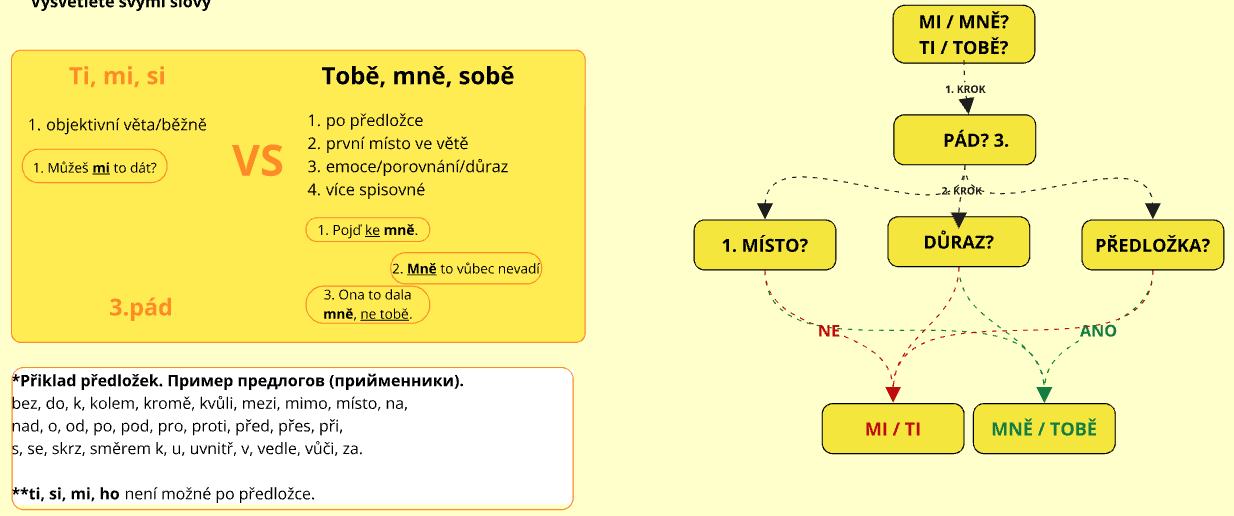
\includegraphics[scale=0.35]{Resources/usage_of_mne_mi.png}
\caption{Usage of \emph{mně} and \emph{mi}}
\label{fig:usage_of_mne_mi}
\end{figure}

\lecture{22}
To ask someone is the 2nd case: \emph{zeptát se (koho? čeho?)}, to ask about something will be 4th case: 
\emph{zeptát se na (koho? co?)}.

\emph{Véde se mu dobře}. \emph{Jak se ti véde (daří)}.

\lecture{23}
After prepositions we use \emph{něj} and not \emph{jeho}.

\emph{Podívat do (koho? čeho?) knihy} -- to look into something.

Word \emph{chtít se} is usually used in 3rd person with the pronoun in 3rd (komu? čemu?) case to indicate on 
who wants something, e.g. \emph{chtělo se jí spát} -- she wanted to sleep.

Word "asi" means "probably" and doesn't stand in the beginning of the sentence, as it would in English, as it 
Czech the type of words like \emph{prý, snad, možná, patrně} are called "modální částice" (modal particles) and they 
gravitate to the beginning of the sentence, but never stand as the first word.

If we want to say "and after a while, he disappeaded from Alenka's sight", we would say \emph{A po chvíli Alence zmizel} 
means he disappeared on Alenka, i.e. from her sight. As his disappearance is framed from Alenka's point of view.

If we say \emph{podívat na (koho? co?)} then we are looking at the surface of something, e.g. \emph{podívat na obrázek},
if we say \emph{podívat do {koho? čeho?}} then we are looking into something, e.g. \emph{podícat do knihy}.

We could say \emph{co to má byt?} and that means \emph{what could it mean?} in a confused and irritated tone.
We could also say \emph{co to může byt?} and that means \emph{what could it be?} in more of a questioning tone.

\emph{Měřit tři metry na výšku/šířku} -- быть 3 метра по высоте/ширине.

Verb \emph{rozumět} expects a noun in 3rd case (komu? čemu?), that is why it is written in this sentence: 
\emph{(komu? čemu?) Ničemu nerozuměla}.

We say here \emph{zkoušet promluvit na ni} in the form of "trying to reach them" or to "address them" that is 
why preposition \emph{na} is used. If we said \emph{promluvit s ni} that would mean that a mutual conversation, 
i.e. a dialogue, is going.

We say here \emph{třast se (s kým? s čým) strahy} instead of \emph{třast od (koho? čeho?) strahu} as here we are 
trying to say \emph{tremble with fear}.
In Czech language, emotions that come with verbs with the logical "with" preposition between them force the emotion 
nouns to be in the 7th case without any preposition, e.g.
\begin{itemize}
    \item \emph{Třást se strachy} -- to shake with fear.
    \item \emph{Smát se radostí} -- to laugh with joy.
    \item \emph{Plakat štěstím} -- to cry with happiness.
    \item \emph{Červenat se studem} -- to blush with shame.
\end{itemize}

Emotions that are used in 2nd case with the preposition \emph{od} before them, usually mean to run away from that emotion, 
i.e. it demands logical "from" or "out of" preposition like a reason, e.g.
\begin{itemize}
    \item \emph{Utekl od strachu} -- he ran away out of fear (fear as the trigger/reason for fleeing).
    \item \emph{Zbledl od strachu} -- he went pale from fear.
\end{itemize}

\emph{Co nejdál} means "as far as possible", in Czech \emph{co + nej-<přídavná jméno>} means "as... as possible", 
e.g. \emph{co nejdřív} -- as soon as possible.

\emph{Je ti zima?} -- are you cold?.

\emph{Dostat cenu} -- means to get an award/prize.

\emph{Blahopřát} requires preposition \emph{k} after itself and the noun that comes after should be in the 3rd case, 
e.g. \emph{blahopřát k narozeninám}.

\emph{Musíme domů} means "have to go home", \emph{domů} indicates a direction, that is why if we would have said 
\emph{musíme být doma} that would mean that "we have to be at home" (e.g. by certain time).





\end{document}
